\documentclass[a4paper,justification=full]{article}

\renewcommand{\familydefault}{\sfdefault}
%include packages
%====================== PACKAGES ======================

\usepackage[table,xcdraw]{xcolor}
\usepackage{fancyhdr}
\usepackage{titlesec}

\usepackage[english]{babel}
%pour gérer les positionnement d'images
\usepackage{svg}
\usepackage{float}
\usepackage{amsmath}
\usepackage{tikz,graphicx}
\usepackage[colorinlistoftodos]{todonotes}
\usepackage{url}
%pour les informations sur un document compilé en PDF et les liens externes / internes
\usepackage{hyperref}
%pour la mise en page des tableaux
\usepackage{array}
\usepackage{tabularx}
\usepackage{multirow}
%pour utiliser \floatbarrier
%\usepackage{placeins}
%\usepackage{floatrow}
%espacement entre les lignes
\usepackage{setspace}
%modifier la mise en page de l'abstract
\usepackage{abstract}
%police et mise en page (marges) du document
\usepackage[T1]{fontenc}
\usepackage[top=2cm, bottom=2cm, left=2cm, right=2cm]{geometry}
%Pour les galerie d'images
\usepackage{subfigure}
%custom package
%espacement entre les lignes d'un tableau
\renewcommand{\arraystretch}{1.5}

%régler l'espacement entre les lignes
\newcommand{\HRule}{\rule{\linewidth}{0.5mm}}


% liste des auteurs
\newcommand{\authorlist}[0]{4A GPSE, Darrys ABDELKRIM, Raimundo Vitor DE SOUSA CARDOSO, \\Florian KRASULJA, Alexandre MAILLET}


%barre pieds de page
\renewcommand{\footrulewidth}{0.6pt}


%Création de la commande pour le sommaire
\makeatletter
\newcommand*{\tableofcontentssummary}{%
  \begingroup
    \value{tocdepth}=1\relax
    \@fileswfalse
    \renewcommand*{\contentsname}{Summary}%
    \tableofcontents
  \endgroup
}
\makeatother


%tabulation
\newcommand\tab[1][0.5cm]{\hspace*{#1}}


%luckyLux
\newcommand{\forest}{\textit{Forest Watch}}

%to define the current file directory
\usepackage{currfile}
%to generate lipsum text
\usepackage{lipsum}
%to get lhe last page
\usepackage{lastpage}
%source
\usepackage[backend=biber,style=numeric,citestyle=authoryear]{biblatex}

\usepackage{enumitem}
\usepackage{listings}


\hypersetup{
  citebordercolor=white,
  filebordercolor=white,
  linkbordercolor=white,
}
\bibliography{test.bib}

%====================== INFORMATION ET REGLES ======================

%rajouter les numérotation pour les \paragraphe et \subparagraphe
\setcounter{secnumdepth}{4}
\setcounter{tocdepth}{4}


\hypersetup{							% Information sur le document
pdfauthor = {\authorlist},			% Auteurs
pdftitle = {},
pdfsubject = {Forest Watch},		% Sujet
pdfkeywords = {},	% Mots-clefs
pdfstartview= {FitH}
}					% ajuste la page à la largueur de l'écran
%pdfcreator = {MikTeX},% Logiciel qui a crée le document
%pdfproducer = {}} % Société avec produit le logiciel

%======================== DEBUT DU DOCUMENT ========================

\begin{document}

%page de garde
\begin{titlepage}
\begin{center}

%logo de l'université

\includegraphics[width=0.25\textwidth]{./titre/universite.jpg}
\hfill
\hfill
%logo de polytech

\includegraphics[width=0.35\textwidth]{./titre/polytech.jpg}~\\[2.5cm]


%logo du thème du document
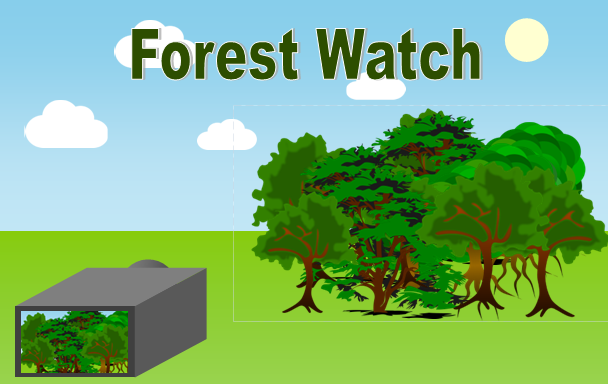
\includegraphics[width=0.8\textwidth]{./titre/logo.png}~\\[1cm]

\textsc{\Large }\\[0.1cm]

% Title
\HRule\\[0.2cm]
{\huge\bfseries Technical Specifications\\
[0.4cm] }

\HRule\\[0.8cm]

% Auteur sur la page principale
\vfill
\begin{minipage}{0.4\textwidth}
    \begin{flushleft} \large
        \emph{}\\
        Darrys \textsc{ABDELKRIM}\\
        Raimundo Vitor \textsc{DE SOUSA CARDOSO}\\
        Florian \textsc{KRASULJA}\\
        Alexandre \textsc{MAILLET}\\
        Engineering student, \textsc{4A GPSE}
    \end{flushleft}
\end{minipage}
% Client et référent sur la page principale
\begin{minipage}{0.4\textwidth}
    \begin{flushright} \large
        Rodolphe \textsc{WEBER}\\
        Teacher in Embedded Systems\\
        Jury chairman
    \end{flushright}
\end{minipage}

\vfill

% Bas de page (date)
{\large  \today}

\end{center}
\end{titlepage}

%style du document
%des paramètre
\onehalfspacing{}
\pagestyle{fancy}
\fancyhf{}

%tête de page
\chead{Capability Development Document}
\lhead{\raisebox{-0.6cm}{
\includegraphics[scale=0.30]{./titre/polytech}}}%logo au centre du pied de page 
\rhead{\today}

%pied de page
\lfoot{\authorlist}
\def\footruleskip{0.2cm}%pour remonter la barre au besoin
\rfoot{Page \thepage{} | \pageref*{LastPage}}
 

%format des sections
\titleformat{\section}
{\normalfont\Large\bfseries}{\thesection.}{1em}{\underline}

%format des sections
\titleformat{\subsection}
{\normalfont\bfseries}{\thesubsection.}{1em}{\underline}

%format des sections
\titleformat{\subsubsection}
{\normalfont\bfseries}{\thesubsubsection.}{1em}{\underline}




%sommaire
\setcounter{page}{1}
%table des matières
\newpage
\renewcommand{\contentsname}{Summary}
%table des matières
% \addcontentsline{toc}{section}{Sommaire}
\tableofcontents{}






%====================== INCLUSION DES PARTIES ======================

\large

%section
%remerciment
\newpage
%le \phantomsection{} permet de regler un bug sur les sommaire qui ne ramène pas a la bonne page
\phantomsection{}
%section sans numéro
\section*{Acknowledgements}
%ajouter quand même la section dans le sommaire
\addcontentsline{toc}{section}{Acknowledgements}


We would like to thank Robotek for lending us the tools to complete this project.
We would also like to thank Rodolphe Weber, our tutor on this project, for his guidance, expertise and support throughout the duration of this project.
Finally, we would like to thank Kamel Ladrouze for providing us with the components we needed for this project.



%intro
%\newpage
%le \phantomsection{} permet de regler un bug sur les sommaire qui ne ramène pas a la bonne page
\phantomsection{}
%section sans numéro
\section*{Technical introduction}
%ajouter quand même la section dans le sommaire
\addcontentsline{toc}{section}{Technical introduction}

The project's goal is to create an autonomous system. It will be able to take two pictures a day in a remote location in a tropical forest for research purposes. The forest is in Gabon, where researchers from the Belgian university of Liège are working on the evolution of trees.
Here is the intended usage scenario:

\begin{figure}[!h]
    \centering
    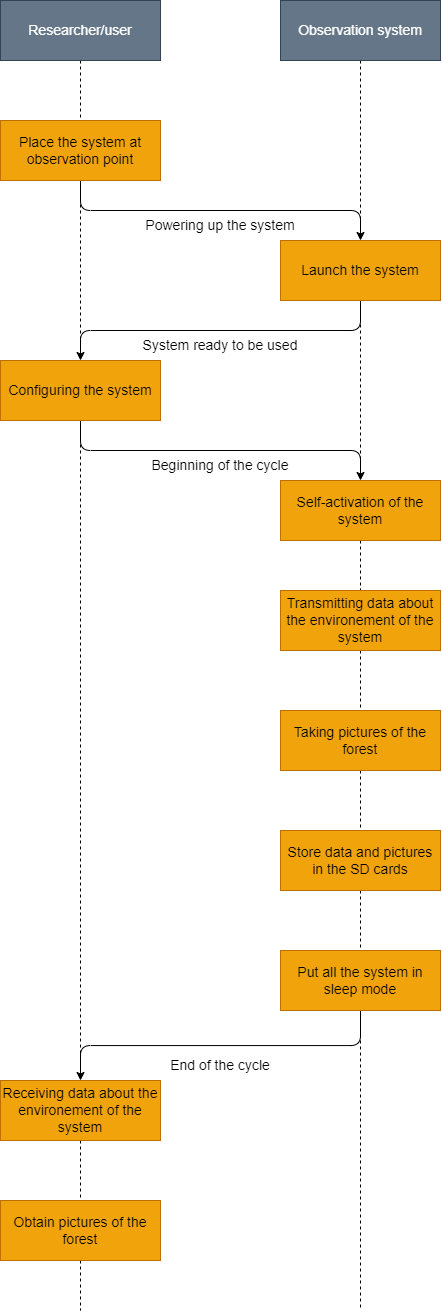
\includegraphics[width=0.5\textwidth]{\currfiledir/figures/usage_scenario.jpg}
    \caption{Picture representing the intended usage scenario for the system.}
\end{figure}

\newpage
%insertion des sections
\newpage
\section{Project description}

\newpage
\subsection{The camera}
The camera is a Lumix DMC-G5. This model has been used in a similar project called micrObs to take pictures of penguins in Antarctica. In this project, the camera has successfully been retro engineered in order to control it automatically. The system to control the camera is explained in the 3.5. part.

\begin{figure}[!h]
    \centering
    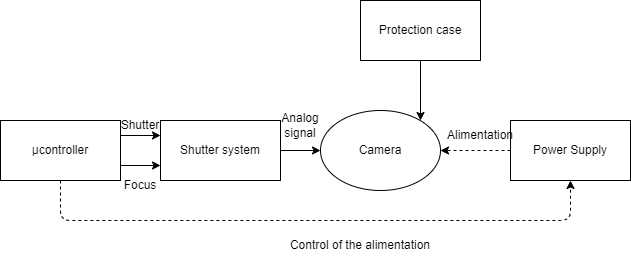
\includegraphics[width=0.9\textwidth]{\currfiledir/figures/camera_diagram.png}
    \caption{Architecture of the system surrounding the camera}
\end{figure}

The camera need a lens to be mounted on it in order to make it work properly. The calculations realized show the lens should be a lens with a focal length between 45 and 150 mm.

Here is the calculation:

\begin{figure}[!h]
    \centering
    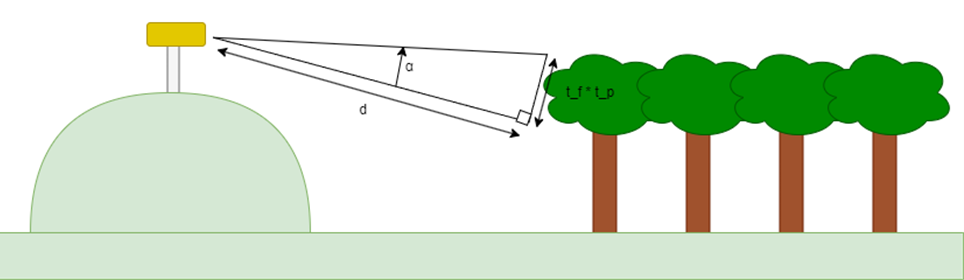
\includegraphics[width=0.85\textwidth]{\currfiledir/figures/calculation_schema.png}
    \caption{Schematic to calculate the focal length for the camera.}
\end{figure}

\noindent\(\alpha\): lens angle of the field of a (to calculate)\\
\(d\): distance between our system and trees (equal to 300 metres)\\
\(t_f\): size of a leaf, estimated to be 5,5 centimetres.\\
\(t_p\): height of the image, which corresponds to 1024 pixels.\\

\noindent According to the trigonometric formulas: \(\alpha=arctan\left(\frac{t_f*t_p}{d}\right)=32,4\textdegree\)

\newpage
%Schematic of different focal lengths
\begin{figure}[!h]
    \centering
    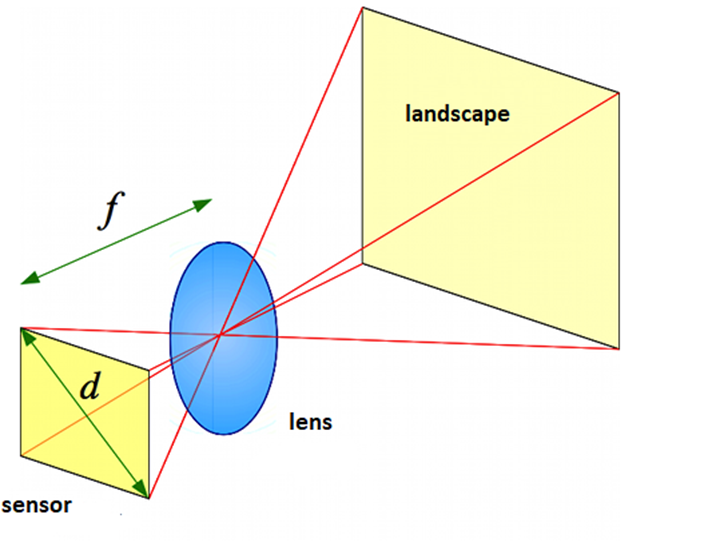
\includegraphics[width=0.75\textwidth]{\currfiledir/figures/calculation.png}
    \caption{Link between angle of view and focal length}
    \cite{focal_length}
\end{figure}

The field of view angle \((\alpha\)) horizontally, corresponding to the length (L) of the sensor, is given by the following formula:
% f=L/(2*tan⁡(α/2) )
\begin{equation}
    f=\frac{L}{2*tan\left(\frac{\alpha}{2}\right)}
\end{equation}

\noindent Where:\\
L: length of the sensor in mm\\
f: focal distance of the lens in mm\\
\(\alpha\): lens angle of the field of view\\
It is obtained: f = 117 mm\\

The equivalent focal length of a Micro 4/3 lens with a field of view of 32.4 degrees is approximately 117 mm.\\


\noindent According to the graph above, we should choose a lens between 100 and 200 mm. The smaller the angle of view (high focal length), the greater the magnification (long focal lengths will give the impression of being closer to the scene captured).\\
Our goal is not to visualize each leaf but each branch so a lens with a focal length of 175 mm will be sufficient for our project.\\
We have therefore selected this objective: \url{https://www.m43lenses.com/panasonic-45-175mm-f4-5.6/}
\newpage
\subsection{Use case}

% \begin{figure}[!h]
%     \centering
%     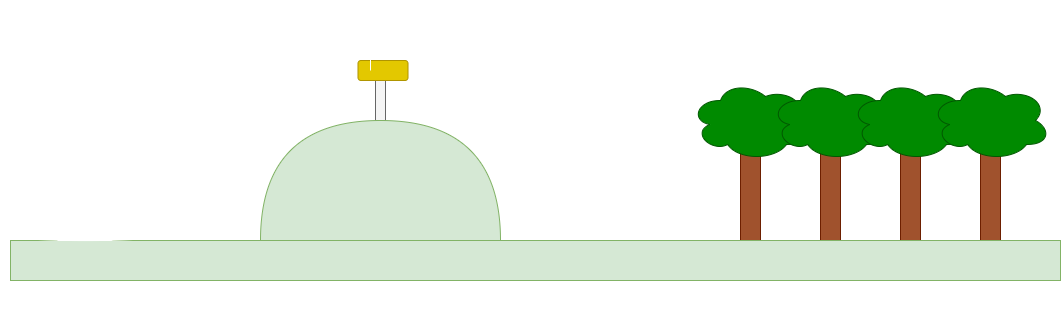
\includegraphics[width=1\textwidth]{\currfiledir/figures/use_case.png}
%     \caption{Use case of the system}
%     \label{fig:forest2}
% \end{figure}


The use case would be as following:
The researchers come once to install the system on a pole on a hill, in front of the group of trees they want to observe. The system would then be placed in the desired location within the forest. The system would be sending data to researchers to ensure that it is functioning properly and that the pictures being taken are of high quality. After 3 months, the researchers would return to the forest to retrieve the system, the stored pictures, and logs about the system state. Then, the researchers would be able to analyse the images.


\newpage
\begin{figure}[!h]
    \centering
    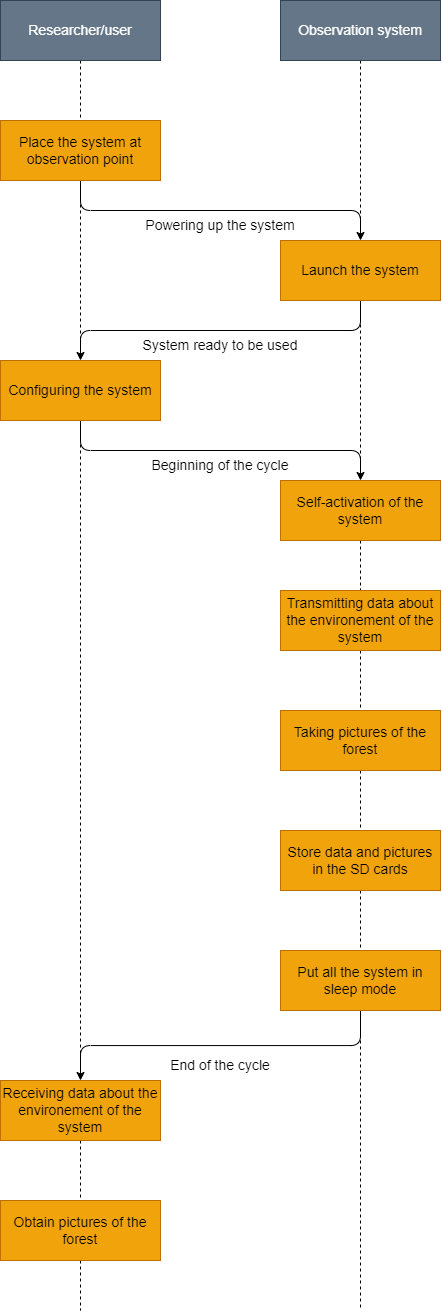
\includegraphics[height=0.95\textheight]{\currfiledir/figures/usage_scenario.png}
    \caption{Picture representing the intended usage scenario for the system.}
\end{figure}

\newpage

\subsection{Functional specifications}

\begin{figure}[!h]
    \centering
    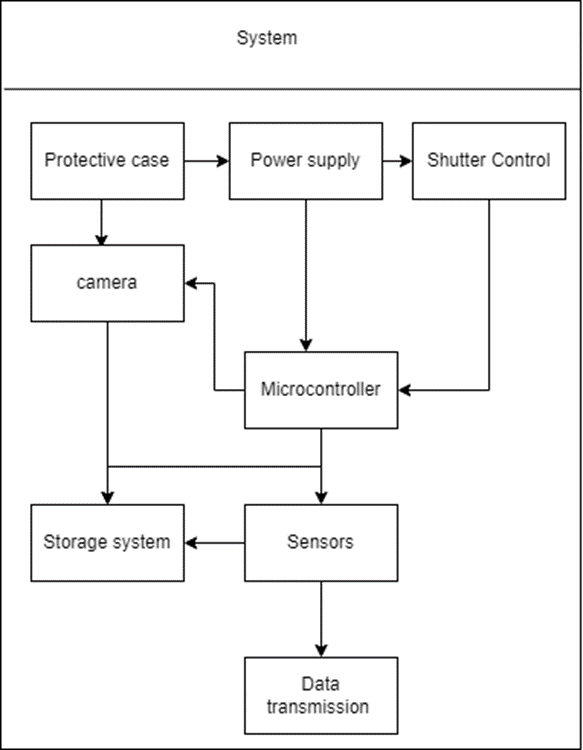
\includegraphics[height=0.5\textheight]{\currfiledir/figures/system.png}
    \caption{Schematic showing different functions interacting inside of the system}
\end{figure}

The diagram illustrates the interconnectivity of these functions, highlighting the relationships and data flow between them. To create a functional system, it is important to ensure that these components are properly integrated and configured to meet the specified technical requirements.

\newpage
\begin{table}[!h]
	\centering
	\begin{tabular}{|c|c|c|c|c|c|}
		\hline
		\rowcolor[HTML]{BFBFBF}
		x                                                  &
		Function                                           &
		Sub-function                                       &
		Criterion                                          &
		Value                                              &
		Flexibility                                          \\ \hline
		F1                                                 &
		\cellcolor[HTML]{CC99FF}Take photos                &
		                                                   &
		                                                   &
		                                                   &
		\cellcolor[HTML]{FFFFFF}{\color[HTML]{FFFFFF} }      \\ \hline
		F1.1                                               &
		                                                   &
		\cellcolor[HTML]{8EA9DB}\begin{tabular}[c]{@{}c@{}}Internal camera \\settings\end{tabular}  &
		                                                   &
		                                                   &
		\\ \hline
		C1.1.1                                             &
		                                                   &
		                                                   &
		\cellcolor[HTML]{A9D08E}Frequency                  &
		\cellcolor[HTML]{FFD966}Once                       &
		\cellcolor[HTML]{ED7D31}2                            \\ \hline
		F1.2                                               &
		                                                   &
		\cellcolor[HTML]{8EA9DB}\begin{tabular}[c]{@{}c@{}}Taking\\ photos regularly\end{tabular}  &
		                                                   &
		                                                   &
		\\ \hline
		C1.2.1                                             &
		                                                   &
		                                                   &
		\cellcolor[HTML]{A9D08E}Frequency                  &
		\cellcolor[HTML]{FFD966}\begin{tabular}[c]{@{}c@{}}2 times a\\ day\end{tabular}  &
		\cellcolor[HTML]{ED7D31}0                            \\ \hline
		F1.3                                               &
		                                                   &
		\cellcolor[HTML]{8EA9DB}\begin{tabular}[c]{@{}c@{}}Taking high-\\ quality photos\end{tabular}  &
		                                                   &
		                                                   &
		\\ \hline
		C1.3.1                                             &
		                                                   &
		                                                   &
		\cellcolor[HTML]{A9D08E}Resolution                 &
		\cellcolor[HTML]{FFD966}1920x1080                    &
		\cellcolor[HTML]{ED7D31}0                            \\ \hline
		C1.3.2                                             &
		                                                   &
		\multicolumn{1}{l|}{}                              &
		\cellcolor[HTML]{A9D08E}Distance                   &
		\cellcolor[HTML]{FFD966}\begin{tabular}[c]{@{}c@{}}300 meters\end{tabular}  &
		\cellcolor[HTML]{ED7D31}0                            \\ \hline
		C1.3.3                                             &
		                                                   &
		\multicolumn{1}{l|}{}                              &
		\cellcolor[HTML]{A9D08E}Fields of view             &
		\cellcolor[HTML]{FFD966}\begin{tabular}[c]{@{}c@{}}32.4°\end{tabular}  &
		\cellcolor[HTML]{ED7D31}1                            \\ \hline 
		F2                                                 &
		\cellcolor[HTML]{CC99FF}\begin{tabular}[c]{@{}c@{}}Possessing an extended\\ battery life\end{tabular}  &
		                                                   &
		                                                   &
		                                                   &
		\\ \hline
		F2.1                                               &
		                                                   &
		\cellcolor[HTML]{8EA9DB}\begin{tabular}[c]{@{}c@{}}Possessing an extended \\battery life\end{tabular}  &
		                                                   &
		                                                   &
		\\ \hline
		C2.1.1                                             &
		                                                   &
		                                                   &
		\cellcolor[HTML]{A9D08E}\begin{tabular}[c]{@{}c@{}}Desired uptime\end{tabular}  &
		\cellcolor[HTML]{FFD966}\(\approx\) 1 year                   &
		\cellcolor[HTML]{ED7D31}1                            \\ \hline
		F3                                                 &
		\cellcolor[HTML]{CC99FF}Storing data               &
		                                                   &
		                                                   &
		                                                   &
		\\ \hline
		F3.1                                               &
		                                                   &
		\cellcolor[HTML]{8EA9DB}Store photos               &
		                                                   &
		                                                   &
		\\ \hline
		C3.1.1                                             &
		                                                   &
		                                                   &
		\cellcolor[HTML]{A9D08E}\begin{tabular}[c]{@{}c@{}}Picture-dedicated \\storage space\end{tabular}  &
		\cellcolor[HTML]{FFD966}\textgreater 16 Go         &
		\cellcolor[HTML]{ED7D31}1                            \\ \hline
		F3.2                                               &
		                                                   &
		\cellcolor[HTML]{8EA9DB}\begin{tabular}[c]{@{}c@{}}Storing  \\ information on \\ the device state\end{tabular} &
		                                                   &
		                                                   &
		\\ \hline
		C3.2.1                                             &
		                                                   &
		                                                   &
		\cellcolor[HTML]{A9D08E}\begin{tabular}[c]{@{}c@{}}Information-dedicated \\ storage  \\ space\end{tabular} &
		\cellcolor[HTML]{FFD966}16 Mo                      &
		\cellcolor[HTML]{ED7D31}3                            \\ \hline
		C3.2.2                                             &
		                                                   &
		                                                   &
		\cellcolor[HTML]{A9D08E}\begin{tabular}[c]{@{}c@{}}Logging period\end{tabular} &
		\cellcolor[HTML]{FFD966}\(\approx\) 1 months                 &
		\cellcolor[HTML]{ED7D31}3                            \\ \hline
		F4                                                 &
		\cellcolor[HTML]{CC99FF}\begin{tabular}[c]{@{}c@{}}Conveying system \\status information\end{tabular} &
		                                                   &
		                                                   &
		                                                   &
		\\ \hline
		F4.1                                               &
		                                                   &
		\cellcolor[HTML]{8EA9DB}Collecting information             &
		                                                   &
		                                                   &
		\\ \hline
		C4.1.1                                             &
		                                                   &
		                                                   &
		\cellcolor[HTML]{A9D08E}\begin{tabular}[c]{@{}c@{}}Remaining battery\\charge percentage\end{tabular} &
		\cellcolor[HTML]{FFD966}\begin{tabular}[c]{@{}c@{}}Error margin \\ of 10\%\end{tabular} &
		\cellcolor[HTML]{ED7D31}2                            \\ \hline
	\end{tabular}
\end{table}

\newpage

% Please add the following required packages to your document preamble:
% \usepackage{multirow}
% \usepackage[table,xcdraw]{xcolor}
% If you use beamer only pass "xcolor=table" option, i.e. \documentclass[xcolor=table]{beamer}
% Please add the following required packages to your document preamble:
% \usepackage{multirow}
% \usepackage[table,xcdraw]{xcolor}
% If you use beamer only pass "xcolor=table" option, i.e. \documentclass[xcolor=table]{beamer}
\begin{table}[!h]
    \centering
    \begin{tabular}{|c|c|c|c|c|c|}
    \hline
     &
       &
       &
      \cellcolor[HTML]{A9D08E} &
      \cellcolor[HTML]{FFD966}\begin{tabular}[c]{@{}c@{}}0°C to 5\\ 0°C\end{tabular} &
      \cellcolor[HTML]{ED7D31}2 \\ \cline{5-6} 
    \multirow{-2}{*}{C4.1.2} &
      \multirow{-2}{*}{} &
      \multirow{-2}{*}{} &
      \multirow{-2}{*}{\cellcolor[HTML]{A9D08E}Temperature} &
      \cellcolor[HTML]{FFD966}\begin{tabular}[c]{@{}c@{}}Precision \\ of 1°C\end{tabular} &
      \cellcolor[HTML]{ED7D31}0 \\ \hline
    C4.1.3 &
       &
       &
      \cellcolor[HTML]{A9D08E}Humidity &
      \cellcolor[HTML]{FFD966}\begin{tabular}[c]{@{}c@{}}80 to \\ 100\%\end{tabular} &
      \cellcolor[HTML]{ED7D31}2 \\ \hline
    C4.1.4 &
       &
       &
      \cellcolor[HTML]{A9D08E}\begin{tabular}[c]{@{}c@{}}Remaining\\  storage\\  space\end{tabular} &
      \cellcolor[HTML]{FFD966}\begin{tabular}[c]{@{}c@{}}Warning \\ at 90\%\end{tabular} &
      \cellcolor[HTML]{ED7D31}2 \\ \hline
    C4.1.5 &
       &
       &
      \cellcolor[HTML]{A9D08E}\begin{tabular}[c]{@{}c@{}}Device \\ motion\end{tabular} &
      \cellcolor[HTML]{FFD966}\begin{tabular}[c]{@{}c@{}}Precision : \\ ± 1cm | \\ ± 1°\end{tabular} &
      \cellcolor[HTML]{ED7D31}1 \\ \hline
    F4.2 &
       &
      \cellcolor[HTML]{8EA9DB}\begin{tabular}[c]{@{}c@{}}Transmitting \\ data remotely\end{tabular} &
       &
       &
       \\ \hline
    C4.2.1 &
       &
       &
      \cellcolor[HTML]{A9D08E}Range &
      \cellcolor[HTML]{FFD966}\(\geq\) 10km &
      \cellcolor[HTML]{ED7D31}1 \\ \hline
    F5 &
      \cellcolor[HTML]{CC99FF}\begin{tabular}[c]{@{}c@{}}Working in a\\  specific \\ environment\end{tabular} &
       &
       &
       &
       \\ \hline
    F5.1 &
       &
      \cellcolor[HTML]{8EA9DB}\begin{tabular}[c]{@{}c@{}}Resisting Central \\ African climate\end{tabular} &
       &
       &
       \\ \hline
    C5.1.1 &
       &
       &
      \cellcolor[HTML]{A9D08E}\begin{tabular}[c]{@{}c@{}}Humidity \\ and fog\end{tabular} &
      \cellcolor[HTML]{FFD966}\begin{tabular}[c]{@{}c@{}}\textgreater 90\% of \\ humidity\end{tabular} &
      \cellcolor[HTML]{ED7D31}0 \\ \hline
    C5.1.2 &
       &
       &
      \cellcolor[HTML]{A9D08E}Temperature &
      \cellcolor[HTML]{FFD966}20°C to 35°C &
      \cellcolor[HTML]{ED7D31}0 \\ \hline
    C5.1.3 &
       &
       &
      \cellcolor[HTML]{A9D08E}Rain &
      \cellcolor[HTML]{FFD966}\begin{tabular}[c]{@{}c@{}}equivalent to\\ IPX4\end{tabular} &
      \cellcolor[HTML]{ED7D31}0 \\ \hline
    \cellcolor[HTML]{FFFFFF}F5.2 &
      \cellcolor[HTML]{FFFFFF} &
      \cellcolor[HTML]{8EA9DB}Size &
       &
       &
       \\ \hline
    \cellcolor[HTML]{FFFFFF}C5.2.1 &
      \cellcolor[HTML]{FFFFFF} &
       &
      \cellcolor[HTML]{A9D08E}Dimensions &
      \cellcolor[HTML]{FFD966}200x300x150 mm &
      \cellcolor[HTML]{ED7D31}2 \\ \hline
    \cellcolor[HTML]{FFFFFF}F5.3 &
      \cellcolor[HTML]{FFFFFF} &
      \cellcolor[HTML]{8EA9DB}Weight &
       &
       &
       \\ \hline
    \cellcolor[HTML]{FFFFFF}C5.3.1 &
      \cellcolor[HTML]{FFFFFF} &
       &
      \cellcolor[HTML]{A9D08E}Mass &
      \cellcolor[HTML]{FFD966}4 kg &
      \cellcolor[HTML]{ED7D31}1 \\ \hline
    \cellcolor[HTML]{FFFFFF}F5.4 &
      \cellcolor[HTML]{FFFFFF} &
      \cellcolor[HTML]{8EA9DB}\begin{tabular}[c]{@{}c@{}}Installation\end{tabular} &
       &
       &
       \\ \hline
    \cellcolor[HTML]{FFFFFF}C5.4.1 &
      \cellcolor[HTML]{FFFFFF} &
       &
      \cellcolor[HTML]{A9D08E}\begin{tabular}[c]{@{}c@{}}Relevant stand \\ or platform\end{tabular} &
      \cellcolor[HTML]{FFD966}??? &
      \cellcolor[HTML]{ED7D31}1 \\ \hline
    \end{tabular}
\end{table}
\tab\tab

\newpage
\section{Compliance Matrix}
\begin{table}[!h]
    \centering
    \begin{tabular}{|c|c|c|c|c|}
    \hline
    Name &
      Criterion &
      Value &
      Test method &
      Conform:   Yes/No/Partially \\ \hline
    C1.2.1 &
      Photo   acquisition frequency &
      2 times a   day &
      \begin{tabular}[c]{@{}c@{}}Let the system run and \\ see if the system can \\ take pictures at various \\ pre-configured hours\end{tabular} &
       \\ \hline
    C1.3.1 &
      Photo   resolution &
      1 branch/pixel   at 300m &
      Outdoor tests &
       \\ \hline
    C1.3.2 &
      Device   uptime &
      1 year &
      \begin{tabular}[c]{@{}c@{}}Let the system run during \\ a period to measure \\ the consumption during \\ this period\end{tabular} &
       \\ \hline
    C2.1.1 &
      Logging   effectiveness &
      * &
      \begin{tabular}[c]{@{}c@{}}Let the system run \\ and verify in the SD card \\ if the logs are effectively \\ written\end{tabular} &
       \\ \hline
    C3.1.1 &
      Remaining   uptime on battery &
      ±10\% &
      \begin{tabular}[c]{@{}c@{}}Let the system run \\ and verify if the calculus \\ realized by the device \\ are correct\end{tabular} &
       \\ \hline
    C4.1.1 &
      Temperature   measures &
      1°C &
      \begin{tabular}[c]{@{}c@{}}Tests with appropriated \\ equipment\end{tabular} &
       \\ \hline
    C4.1.4 &
      Device   motion warning &
      2 cm/1° &
      \begin{tabular}[c]{@{}c@{}}Manual movement \\ input\end{tabular} &
       \\ \hline
    C4.1.5 &
      Distance   de transmission &
      10 km &
      Long distance tests &
      \begin{tabular}[c]{@{}c@{}}Partially\end{tabular} \\ \hline
    C4.2.1 &
      Humidity   resistance &
      \textgreater 90\% &
      To be determined &
       \\ \hline
    C5.1.1 &
      Temperature   resistance &
      20 - 40°C &
      \begin{tabular}[c]{@{}c@{}}Exposing the \\ temperature sensors to \\ known temperatures and \\ read the value read by \\ the microcontroller\end{tabular} &
       \\ \hline
    C5.1.2 &
      Rain   resistance &
      IP X4   equivalent &
      \begin{tabular}[c]{@{}c@{}}Leaving the box \\ under the shower \\ for 10 minutes\end{tabular} &
       \\ \hline
    C5.1.3 &
      Small   dimensions &
      212 x 149   x 93 mm &
      Measurements &
       \\ \hline
    \cellcolor[HTML]{FFFFFF}C5.2.1 &
      Overall   mass &
      4 kg &
      " &
       \\ \hline
    \end{tabular}
  \end{table}

The compliance matrix is a table with outlines various criteria or specifications that a device or system must meet, along with their corresponding values and test methods.

\newpage
\section{Project description}

\newpage
\subsection{The camera}
The camera is a Lumix DMC-G5. This model has been used in a similar project called micrObs to take pictures of penguins in Antarctica. In this project, the camera has successfully been retro engineered in order to control it automatically. The system to control the camera is explained in the 3.5. part.

\begin{figure}[!h]
    \centering
    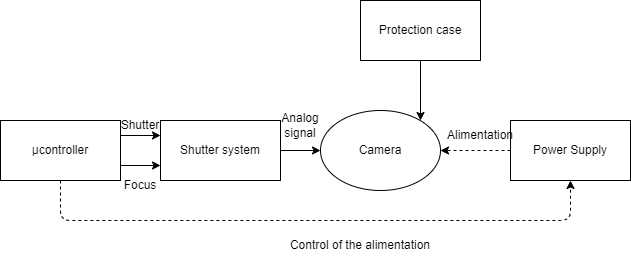
\includegraphics[width=0.9\textwidth]{\currfiledir/figures/camera_diagram.png}
    \caption{Architecture of the system surrounding the camera}
\end{figure}

The camera need a lens to be mounted on it in order to make it work properly. The calculations realized show the lens should be a lens with a focal length between 45 and 150 mm.

Here is the calculation:

\begin{figure}[!h]
    \centering
    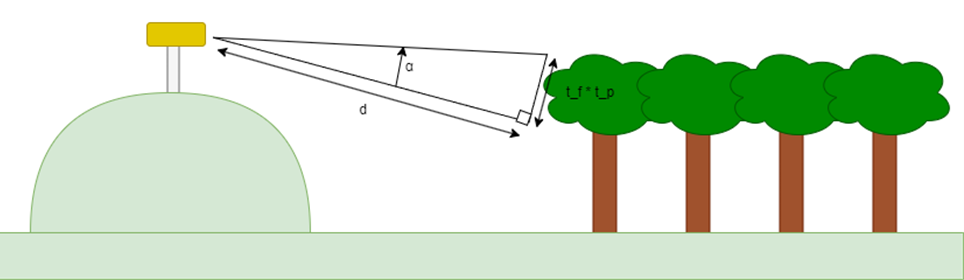
\includegraphics[width=0.85\textwidth]{\currfiledir/figures/calculation_schema.png}
    \caption{Schematic to calculate the focal length for the camera.}
\end{figure}

\noindent\(\alpha\): lens angle of the field of a (to calculate)\\
\(d\): distance between our system and trees (equal to 300 metres)\\
\(t_f\): size of a leaf, estimated to be 5,5 centimetres.\\
\(t_p\): height of the image, which corresponds to 1024 pixels.\\

\noindent According to the trigonometric formulas: \(\alpha=arctan\left(\frac{t_f*t_p}{d}\right)=32,4\textdegree\)

\newpage
%Schematic of different focal lengths
\begin{figure}[!h]
    \centering
    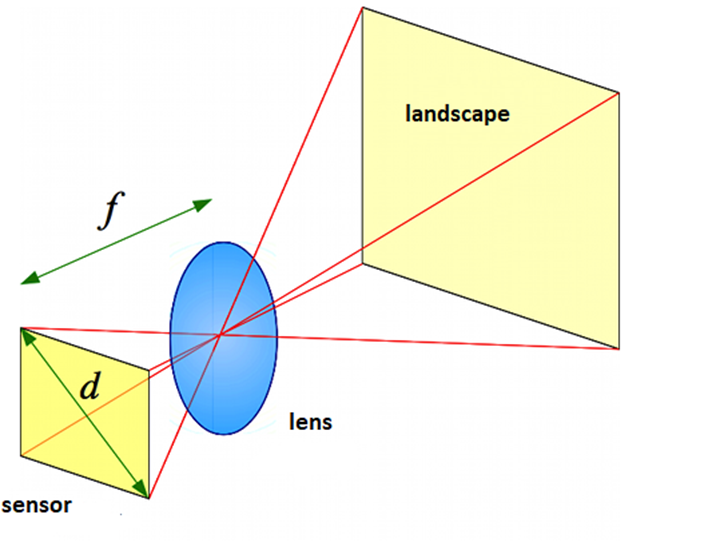
\includegraphics[width=0.75\textwidth]{\currfiledir/figures/calculation.png}
    \caption{Link between angle of view and focal length}
    \cite{focal_length}
\end{figure}

The field of view angle \((\alpha\)) horizontally, corresponding to the length (L) of the sensor, is given by the following formula:
% f=L/(2*tan⁡(α/2) )
\begin{equation}
    f=\frac{L}{2*tan\left(\frac{\alpha}{2}\right)}
\end{equation}

\noindent Where:\\
L: length of the sensor in mm\\
f: focal distance of the lens in mm\\
\(\alpha\): lens angle of the field of view\\
It is obtained: f = 117 mm\\

The equivalent focal length of a Micro 4/3 lens with a field of view of 32.4 degrees is approximately 117 mm.\\


\noindent According to the graph above, we should choose a lens between 100 and 200 mm. The smaller the angle of view (high focal length), the greater the magnification (long focal lengths will give the impression of being closer to the scene captured).\\
Our goal is not to visualize each leaf but each branch so a lens with a focal length of 175 mm will be sufficient for our project.\\
We have therefore selected this objective: \url{https://www.m43lenses.com/panasonic-45-175mm-f4-5.6/}
\newpage
\subsection{Use case}

% \begin{figure}[!h]
%     \centering
%     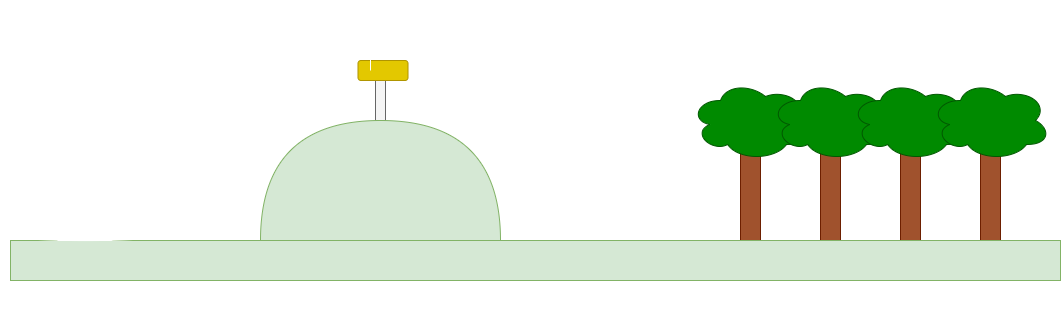
\includegraphics[width=1\textwidth]{\currfiledir/figures/use_case.png}
%     \caption{Use case of the system}
%     \label{fig:forest2}
% \end{figure}


The use case would be as following:
The researchers come once to install the system on a pole on a hill, in front of the group of trees they want to observe. The system would then be placed in the desired location within the forest. The system would be sending data to researchers to ensure that it is functioning properly and that the pictures being taken are of high quality. After 3 months, the researchers would return to the forest to retrieve the system, the stored pictures, and logs about the system state. Then, the researchers would be able to analyse the images.


\newpage
\begin{figure}[!h]
    \centering
    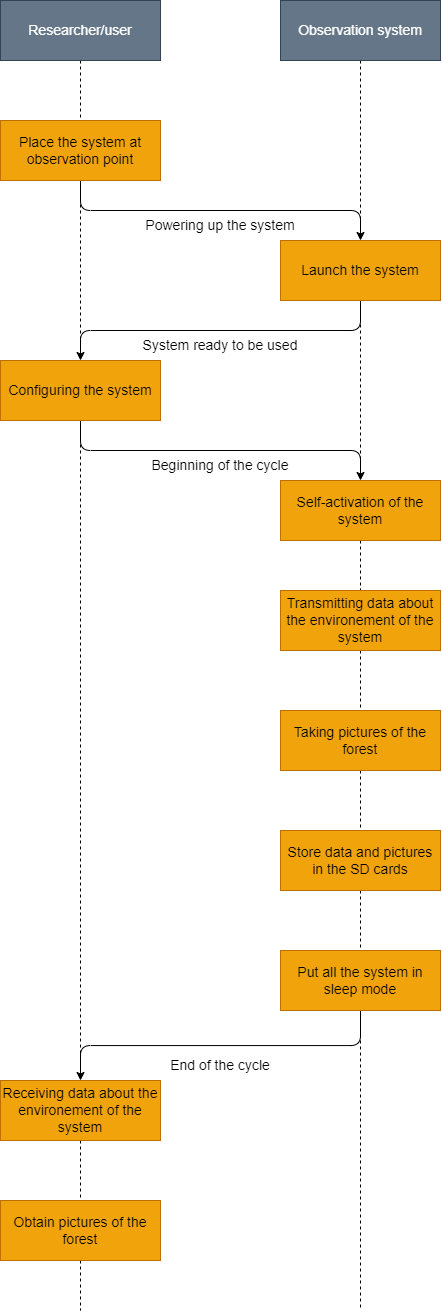
\includegraphics[height=0.95\textheight]{\currfiledir/figures/usage_scenario.png}
    \caption{Picture representing the intended usage scenario for the system.}
\end{figure}

\newpage

\subsection{Functional specifications}

\begin{figure}[!h]
    \centering
    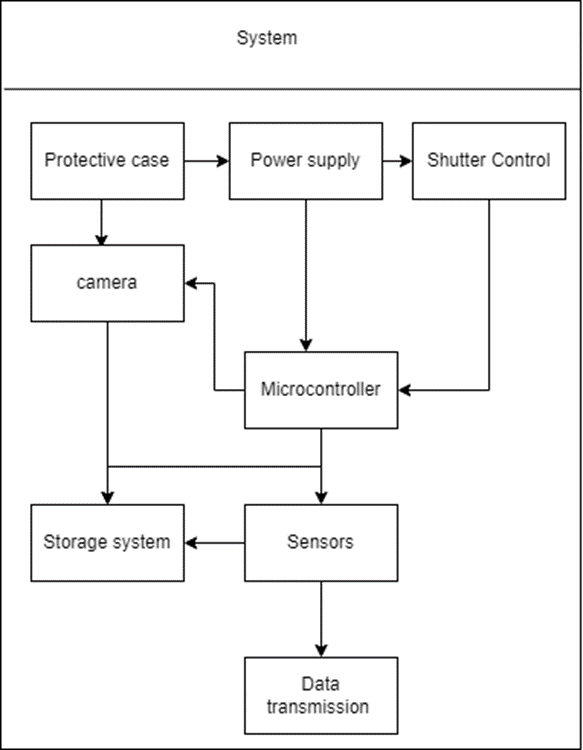
\includegraphics[height=0.5\textheight]{\currfiledir/figures/system.png}
    \caption{Schematic showing different functions interacting inside of the system}
\end{figure}

The diagram illustrates the interconnectivity of these functions, highlighting the relationships and data flow between them. To create a functional system, it is important to ensure that these components are properly integrated and configured to meet the specified technical requirements.

\newpage
\begin{table}[!h]
	\centering
	\begin{tabular}{|c|c|c|c|c|c|}
		\hline
		\rowcolor[HTML]{BFBFBF}
		x                                                  &
		Function                                           &
		Sub-function                                       &
		Criterion                                          &
		Value                                              &
		Flexibility                                          \\ \hline
		F1                                                 &
		\cellcolor[HTML]{CC99FF}Take photos                &
		                                                   &
		                                                   &
		                                                   &
		\cellcolor[HTML]{FFFFFF}{\color[HTML]{FFFFFF} }      \\ \hline
		F1.1                                               &
		                                                   &
		\cellcolor[HTML]{8EA9DB}\begin{tabular}[c]{@{}c@{}}Internal camera \\settings\end{tabular}  &
		                                                   &
		                                                   &
		\\ \hline
		C1.1.1                                             &
		                                                   &
		                                                   &
		\cellcolor[HTML]{A9D08E}Frequency                  &
		\cellcolor[HTML]{FFD966}Once                       &
		\cellcolor[HTML]{ED7D31}2                            \\ \hline
		F1.2                                               &
		                                                   &
		\cellcolor[HTML]{8EA9DB}\begin{tabular}[c]{@{}c@{}}Taking\\ photos regularly\end{tabular}  &
		                                                   &
		                                                   &
		\\ \hline
		C1.2.1                                             &
		                                                   &
		                                                   &
		\cellcolor[HTML]{A9D08E}Frequency                  &
		\cellcolor[HTML]{FFD966}\begin{tabular}[c]{@{}c@{}}2 times a\\ day\end{tabular}  &
		\cellcolor[HTML]{ED7D31}0                            \\ \hline
		F1.3                                               &
		                                                   &
		\cellcolor[HTML]{8EA9DB}\begin{tabular}[c]{@{}c@{}}Taking high-\\ quality photos\end{tabular}  &
		                                                   &
		                                                   &
		\\ \hline
		C1.3.1                                             &
		                                                   &
		                                                   &
		\cellcolor[HTML]{A9D08E}Resolution                 &
		\cellcolor[HTML]{FFD966}1920x1080                    &
		\cellcolor[HTML]{ED7D31}0                            \\ \hline
		C1.3.2                                             &
		                                                   &
		\multicolumn{1}{l|}{}                              &
		\cellcolor[HTML]{A9D08E}Distance                   &
		\cellcolor[HTML]{FFD966}\begin{tabular}[c]{@{}c@{}}300 meters\end{tabular}  &
		\cellcolor[HTML]{ED7D31}0                            \\ \hline
		C1.3.3                                             &
		                                                   &
		\multicolumn{1}{l|}{}                              &
		\cellcolor[HTML]{A9D08E}Fields of view             &
		\cellcolor[HTML]{FFD966}\begin{tabular}[c]{@{}c@{}}32.4°\end{tabular}  &
		\cellcolor[HTML]{ED7D31}1                            \\ \hline 
		F2                                                 &
		\cellcolor[HTML]{CC99FF}\begin{tabular}[c]{@{}c@{}}Possessing an extended\\ battery life\end{tabular}  &
		                                                   &
		                                                   &
		                                                   &
		\\ \hline
		F2.1                                               &
		                                                   &
		\cellcolor[HTML]{8EA9DB}\begin{tabular}[c]{@{}c@{}}Possessing an extended \\battery life\end{tabular}  &
		                                                   &
		                                                   &
		\\ \hline
		C2.1.1                                             &
		                                                   &
		                                                   &
		\cellcolor[HTML]{A9D08E}\begin{tabular}[c]{@{}c@{}}Desired uptime\end{tabular}  &
		\cellcolor[HTML]{FFD966}\(\approx\) 1 year                   &
		\cellcolor[HTML]{ED7D31}1                            \\ \hline
		F3                                                 &
		\cellcolor[HTML]{CC99FF}Storing data               &
		                                                   &
		                                                   &
		                                                   &
		\\ \hline
		F3.1                                               &
		                                                   &
		\cellcolor[HTML]{8EA9DB}Store photos               &
		                                                   &
		                                                   &
		\\ \hline
		C3.1.1                                             &
		                                                   &
		                                                   &
		\cellcolor[HTML]{A9D08E}\begin{tabular}[c]{@{}c@{}}Picture-dedicated \\storage space\end{tabular}  &
		\cellcolor[HTML]{FFD966}\textgreater 16 Go         &
		\cellcolor[HTML]{ED7D31}1                            \\ \hline
		F3.2                                               &
		                                                   &
		\cellcolor[HTML]{8EA9DB}\begin{tabular}[c]{@{}c@{}}Storing  \\ information on \\ the device state\end{tabular} &
		                                                   &
		                                                   &
		\\ \hline
		C3.2.1                                             &
		                                                   &
		                                                   &
		\cellcolor[HTML]{A9D08E}\begin{tabular}[c]{@{}c@{}}Information-dedicated \\ storage  \\ space\end{tabular} &
		\cellcolor[HTML]{FFD966}16 Mo                      &
		\cellcolor[HTML]{ED7D31}3                            \\ \hline
		C3.2.2                                             &
		                                                   &
		                                                   &
		\cellcolor[HTML]{A9D08E}\begin{tabular}[c]{@{}c@{}}Logging period\end{tabular} &
		\cellcolor[HTML]{FFD966}\(\approx\) 1 months                 &
		\cellcolor[HTML]{ED7D31}3                            \\ \hline
		F4                                                 &
		\cellcolor[HTML]{CC99FF}\begin{tabular}[c]{@{}c@{}}Conveying system \\status information\end{tabular} &
		                                                   &
		                                                   &
		                                                   &
		\\ \hline
		F4.1                                               &
		                                                   &
		\cellcolor[HTML]{8EA9DB}Collecting information             &
		                                                   &
		                                                   &
		\\ \hline
		C4.1.1                                             &
		                                                   &
		                                                   &
		\cellcolor[HTML]{A9D08E}\begin{tabular}[c]{@{}c@{}}Remaining battery\\charge percentage\end{tabular} &
		\cellcolor[HTML]{FFD966}\begin{tabular}[c]{@{}c@{}}Error margin \\ of 10\%\end{tabular} &
		\cellcolor[HTML]{ED7D31}2                            \\ \hline
	\end{tabular}
\end{table}

\newpage

% Please add the following required packages to your document preamble:
% \usepackage{multirow}
% \usepackage[table,xcdraw]{xcolor}
% If you use beamer only pass "xcolor=table" option, i.e. \documentclass[xcolor=table]{beamer}
% Please add the following required packages to your document preamble:
% \usepackage{multirow}
% \usepackage[table,xcdraw]{xcolor}
% If you use beamer only pass "xcolor=table" option, i.e. \documentclass[xcolor=table]{beamer}
\begin{table}[!h]
    \centering
    \begin{tabular}{|c|c|c|c|c|c|}
    \hline
     &
       &
       &
      \cellcolor[HTML]{A9D08E} &
      \cellcolor[HTML]{FFD966}\begin{tabular}[c]{@{}c@{}}0°C to 5\\ 0°C\end{tabular} &
      \cellcolor[HTML]{ED7D31}2 \\ \cline{5-6} 
    \multirow{-2}{*}{C4.1.2} &
      \multirow{-2}{*}{} &
      \multirow{-2}{*}{} &
      \multirow{-2}{*}{\cellcolor[HTML]{A9D08E}Temperature} &
      \cellcolor[HTML]{FFD966}\begin{tabular}[c]{@{}c@{}}Precision \\ of 1°C\end{tabular} &
      \cellcolor[HTML]{ED7D31}0 \\ \hline
    C4.1.3 &
       &
       &
      \cellcolor[HTML]{A9D08E}Humidity &
      \cellcolor[HTML]{FFD966}\begin{tabular}[c]{@{}c@{}}80 to \\ 100\%\end{tabular} &
      \cellcolor[HTML]{ED7D31}2 \\ \hline
    C4.1.4 &
       &
       &
      \cellcolor[HTML]{A9D08E}\begin{tabular}[c]{@{}c@{}}Remaining\\  storage\\  space\end{tabular} &
      \cellcolor[HTML]{FFD966}\begin{tabular}[c]{@{}c@{}}Warning \\ at 90\%\end{tabular} &
      \cellcolor[HTML]{ED7D31}2 \\ \hline
    C4.1.5 &
       &
       &
      \cellcolor[HTML]{A9D08E}\begin{tabular}[c]{@{}c@{}}Device \\ motion\end{tabular} &
      \cellcolor[HTML]{FFD966}\begin{tabular}[c]{@{}c@{}}Precision : \\ ± 1cm | \\ ± 1°\end{tabular} &
      \cellcolor[HTML]{ED7D31}1 \\ \hline
    F4.2 &
       &
      \cellcolor[HTML]{8EA9DB}\begin{tabular}[c]{@{}c@{}}Transmitting \\ data remotely\end{tabular} &
       &
       &
       \\ \hline
    C4.2.1 &
       &
       &
      \cellcolor[HTML]{A9D08E}Range &
      \cellcolor[HTML]{FFD966}\(\geq\) 10km &
      \cellcolor[HTML]{ED7D31}1 \\ \hline
    F5 &
      \cellcolor[HTML]{CC99FF}\begin{tabular}[c]{@{}c@{}}Working in a\\  specific \\ environment\end{tabular} &
       &
       &
       &
       \\ \hline
    F5.1 &
       &
      \cellcolor[HTML]{8EA9DB}\begin{tabular}[c]{@{}c@{}}Resisting Central \\ African climate\end{tabular} &
       &
       &
       \\ \hline
    C5.1.1 &
       &
       &
      \cellcolor[HTML]{A9D08E}\begin{tabular}[c]{@{}c@{}}Humidity \\ and fog\end{tabular} &
      \cellcolor[HTML]{FFD966}\begin{tabular}[c]{@{}c@{}}\textgreater 90\% of \\ humidity\end{tabular} &
      \cellcolor[HTML]{ED7D31}0 \\ \hline
    C5.1.2 &
       &
       &
      \cellcolor[HTML]{A9D08E}Temperature &
      \cellcolor[HTML]{FFD966}20°C to 35°C &
      \cellcolor[HTML]{ED7D31}0 \\ \hline
    C5.1.3 &
       &
       &
      \cellcolor[HTML]{A9D08E}Rain &
      \cellcolor[HTML]{FFD966}\begin{tabular}[c]{@{}c@{}}equivalent to\\ IPX4\end{tabular} &
      \cellcolor[HTML]{ED7D31}0 \\ \hline
    \cellcolor[HTML]{FFFFFF}F5.2 &
      \cellcolor[HTML]{FFFFFF} &
      \cellcolor[HTML]{8EA9DB}Size &
       &
       &
       \\ \hline
    \cellcolor[HTML]{FFFFFF}C5.2.1 &
      \cellcolor[HTML]{FFFFFF} &
       &
      \cellcolor[HTML]{A9D08E}Dimensions &
      \cellcolor[HTML]{FFD966}200x300x150 mm &
      \cellcolor[HTML]{ED7D31}2 \\ \hline
    \cellcolor[HTML]{FFFFFF}F5.3 &
      \cellcolor[HTML]{FFFFFF} &
      \cellcolor[HTML]{8EA9DB}Weight &
       &
       &
       \\ \hline
    \cellcolor[HTML]{FFFFFF}C5.3.1 &
      \cellcolor[HTML]{FFFFFF} &
       &
      \cellcolor[HTML]{A9D08E}Mass &
      \cellcolor[HTML]{FFD966}4 kg &
      \cellcolor[HTML]{ED7D31}1 \\ \hline
    \cellcolor[HTML]{FFFFFF}F5.4 &
      \cellcolor[HTML]{FFFFFF} &
      \cellcolor[HTML]{8EA9DB}\begin{tabular}[c]{@{}c@{}}Installation\end{tabular} &
       &
       &
       \\ \hline
    \cellcolor[HTML]{FFFFFF}C5.4.1 &
      \cellcolor[HTML]{FFFFFF} &
       &
      \cellcolor[HTML]{A9D08E}\begin{tabular}[c]{@{}c@{}}Relevant stand \\ or platform\end{tabular} &
      \cellcolor[HTML]{FFD966}??? &
      \cellcolor[HTML]{ED7D31}1 \\ \hline
    \end{tabular}
\end{table}
\tab\tab

% \newpage
\section{Project description}

\newpage
\subsection{The camera}
The camera is a Lumix DMC-G5. This model has been used in a similar project called micrObs to take pictures of penguins in Antarctica. In this project, the camera has successfully been retro engineered in order to control it automatically. The system to control the camera is explained in the 3.5. part.

\begin{figure}[!h]
    \centering
    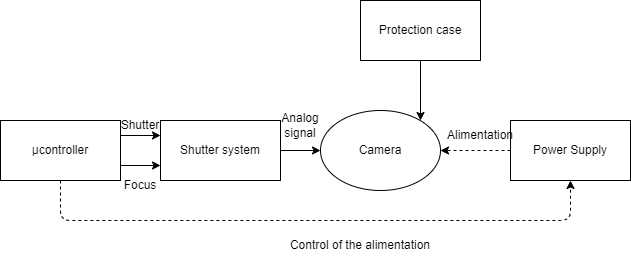
\includegraphics[width=0.9\textwidth]{\currfiledir/figures/camera_diagram.png}
    \caption{Architecture of the system surrounding the camera}
\end{figure}

The camera need a lens to be mounted on it in order to make it work properly. The calculations realized show the lens should be a lens with a focal length between 45 and 150 mm.

Here is the calculation:

\begin{figure}[!h]
    \centering
    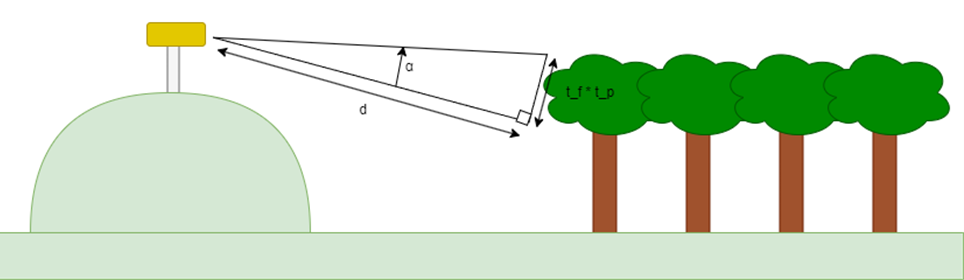
\includegraphics[width=0.85\textwidth]{\currfiledir/figures/calculation_schema.png}
    \caption{Schematic to calculate the focal length for the camera.}
\end{figure}

\noindent\(\alpha\): lens angle of the field of a (to calculate)\\
\(d\): distance between our system and trees (equal to 300 metres)\\
\(t_f\): size of a leaf, estimated to be 5,5 centimetres.\\
\(t_p\): height of the image, which corresponds to 1024 pixels.\\

\noindent According to the trigonometric formulas: \(\alpha=arctan\left(\frac{t_f*t_p}{d}\right)=32,4\textdegree\)

\newpage
%Schematic of different focal lengths
\begin{figure}[!h]
    \centering
    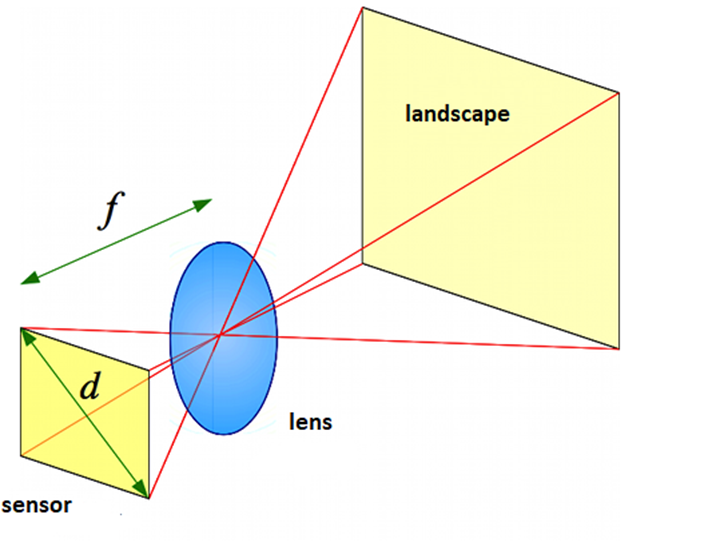
\includegraphics[width=0.75\textwidth]{\currfiledir/figures/calculation.png}
    \caption{Link between angle of view and focal length}
    \cite{focal_length}
\end{figure}

The field of view angle \((\alpha\)) horizontally, corresponding to the length (L) of the sensor, is given by the following formula:
% f=L/(2*tan⁡(α/2) )
\begin{equation}
    f=\frac{L}{2*tan\left(\frac{\alpha}{2}\right)}
\end{equation}

\noindent Where:\\
L: length of the sensor in mm\\
f: focal distance of the lens in mm\\
\(\alpha\): lens angle of the field of view\\
It is obtained: f = 117 mm\\

The equivalent focal length of a Micro 4/3 lens with a field of view of 32.4 degrees is approximately 117 mm.\\


\noindent According to the graph above, we should choose a lens between 100 and 200 mm. The smaller the angle of view (high focal length), the greater the magnification (long focal lengths will give the impression of being closer to the scene captured).\\
Our goal is not to visualize each leaf but each branch so a lens with a focal length of 175 mm will be sufficient for our project.\\
We have therefore selected this objective: \url{https://www.m43lenses.com/panasonic-45-175mm-f4-5.6/}
\newpage
\subsection{Use case}

% \begin{figure}[!h]
%     \centering
%     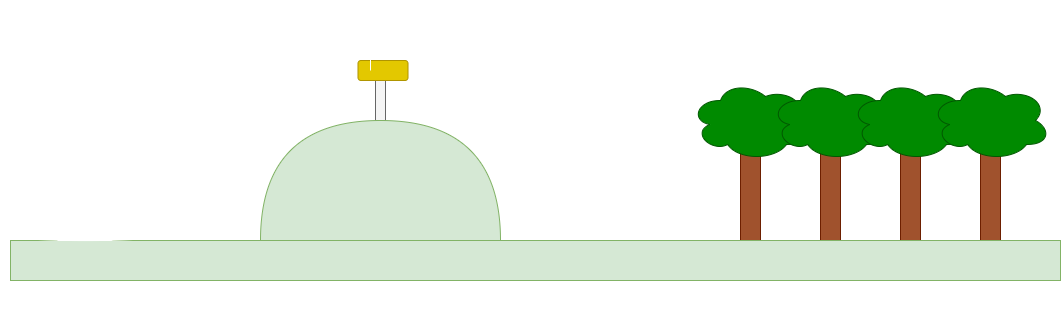
\includegraphics[width=1\textwidth]{\currfiledir/figures/use_case.png}
%     \caption{Use case of the system}
%     \label{fig:forest2}
% \end{figure}


The use case would be as following:
The researchers come once to install the system on a pole on a hill, in front of the group of trees they want to observe. The system would then be placed in the desired location within the forest. The system would be sending data to researchers to ensure that it is functioning properly and that the pictures being taken are of high quality. After 3 months, the researchers would return to the forest to retrieve the system, the stored pictures, and logs about the system state. Then, the researchers would be able to analyse the images.


\newpage
\begin{figure}[!h]
    \centering
    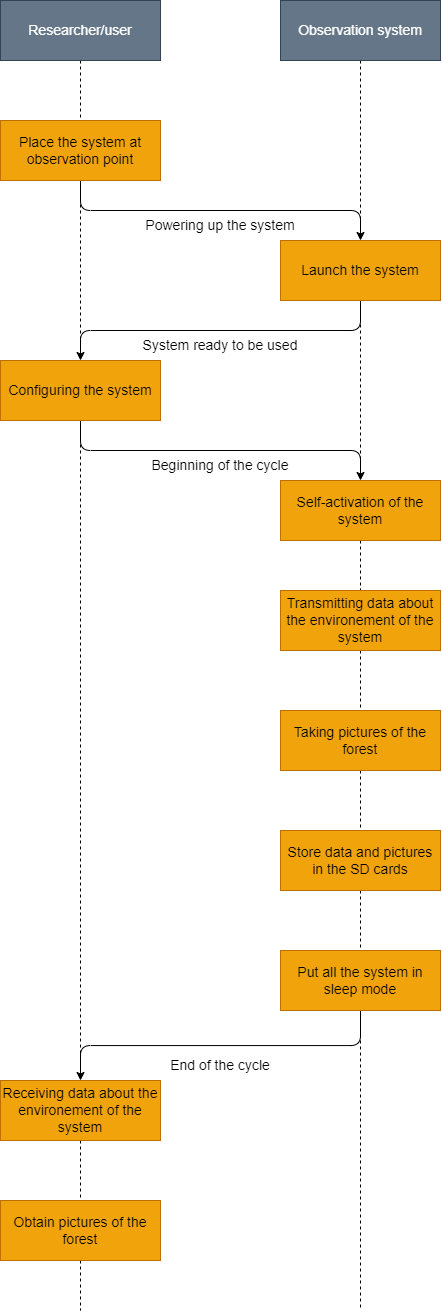
\includegraphics[height=0.95\textheight]{\currfiledir/figures/usage_scenario.png}
    \caption{Picture representing the intended usage scenario for the system.}
\end{figure}

\newpage

\subsection{Functional specifications}

\begin{figure}[!h]
    \centering
    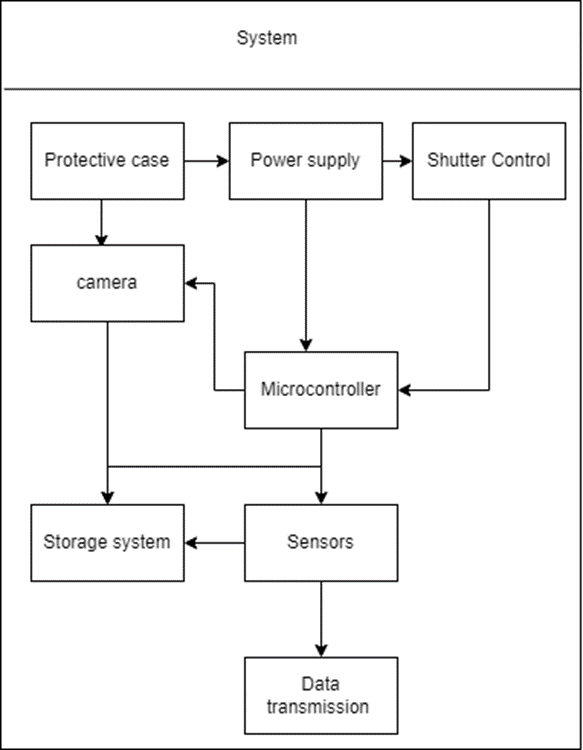
\includegraphics[height=0.5\textheight]{\currfiledir/figures/system.png}
    \caption{Schematic showing different functions interacting inside of the system}
\end{figure}

The diagram illustrates the interconnectivity of these functions, highlighting the relationships and data flow between them. To create a functional system, it is important to ensure that these components are properly integrated and configured to meet the specified technical requirements.

\newpage
\begin{table}[!h]
	\centering
	\begin{tabular}{|c|c|c|c|c|c|}
		\hline
		\rowcolor[HTML]{BFBFBF}
		x                                                  &
		Function                                           &
		Sub-function                                       &
		Criterion                                          &
		Value                                              &
		Flexibility                                          \\ \hline
		F1                                                 &
		\cellcolor[HTML]{CC99FF}Take photos                &
		                                                   &
		                                                   &
		                                                   &
		\cellcolor[HTML]{FFFFFF}{\color[HTML]{FFFFFF} }      \\ \hline
		F1.1                                               &
		                                                   &
		\cellcolor[HTML]{8EA9DB}\begin{tabular}[c]{@{}c@{}}Internal camera \\settings\end{tabular}  &
		                                                   &
		                                                   &
		\\ \hline
		C1.1.1                                             &
		                                                   &
		                                                   &
		\cellcolor[HTML]{A9D08E}Frequency                  &
		\cellcolor[HTML]{FFD966}Once                       &
		\cellcolor[HTML]{ED7D31}2                            \\ \hline
		F1.2                                               &
		                                                   &
		\cellcolor[HTML]{8EA9DB}\begin{tabular}[c]{@{}c@{}}Taking\\ photos regularly\end{tabular}  &
		                                                   &
		                                                   &
		\\ \hline
		C1.2.1                                             &
		                                                   &
		                                                   &
		\cellcolor[HTML]{A9D08E}Frequency                  &
		\cellcolor[HTML]{FFD966}\begin{tabular}[c]{@{}c@{}}2 times a\\ day\end{tabular}  &
		\cellcolor[HTML]{ED7D31}0                            \\ \hline
		F1.3                                               &
		                                                   &
		\cellcolor[HTML]{8EA9DB}\begin{tabular}[c]{@{}c@{}}Taking high-\\ quality photos\end{tabular}  &
		                                                   &
		                                                   &
		\\ \hline
		C1.3.1                                             &
		                                                   &
		                                                   &
		\cellcolor[HTML]{A9D08E}Resolution                 &
		\cellcolor[HTML]{FFD966}1920x1080                    &
		\cellcolor[HTML]{ED7D31}0                            \\ \hline
		C1.3.2                                             &
		                                                   &
		\multicolumn{1}{l|}{}                              &
		\cellcolor[HTML]{A9D08E}Distance                   &
		\cellcolor[HTML]{FFD966}\begin{tabular}[c]{@{}c@{}}300 meters\end{tabular}  &
		\cellcolor[HTML]{ED7D31}0                            \\ \hline
		C1.3.3                                             &
		                                                   &
		\multicolumn{1}{l|}{}                              &
		\cellcolor[HTML]{A9D08E}Fields of view             &
		\cellcolor[HTML]{FFD966}\begin{tabular}[c]{@{}c@{}}32.4°\end{tabular}  &
		\cellcolor[HTML]{ED7D31}1                            \\ \hline 
		F2                                                 &
		\cellcolor[HTML]{CC99FF}\begin{tabular}[c]{@{}c@{}}Possessing an extended\\ battery life\end{tabular}  &
		                                                   &
		                                                   &
		                                                   &
		\\ \hline
		F2.1                                               &
		                                                   &
		\cellcolor[HTML]{8EA9DB}\begin{tabular}[c]{@{}c@{}}Possessing an extended \\battery life\end{tabular}  &
		                                                   &
		                                                   &
		\\ \hline
		C2.1.1                                             &
		                                                   &
		                                                   &
		\cellcolor[HTML]{A9D08E}\begin{tabular}[c]{@{}c@{}}Desired uptime\end{tabular}  &
		\cellcolor[HTML]{FFD966}\(\approx\) 1 year                   &
		\cellcolor[HTML]{ED7D31}1                            \\ \hline
		F3                                                 &
		\cellcolor[HTML]{CC99FF}Storing data               &
		                                                   &
		                                                   &
		                                                   &
		\\ \hline
		F3.1                                               &
		                                                   &
		\cellcolor[HTML]{8EA9DB}Store photos               &
		                                                   &
		                                                   &
		\\ \hline
		C3.1.1                                             &
		                                                   &
		                                                   &
		\cellcolor[HTML]{A9D08E}\begin{tabular}[c]{@{}c@{}}Picture-dedicated \\storage space\end{tabular}  &
		\cellcolor[HTML]{FFD966}\textgreater 16 Go         &
		\cellcolor[HTML]{ED7D31}1                            \\ \hline
		F3.2                                               &
		                                                   &
		\cellcolor[HTML]{8EA9DB}\begin{tabular}[c]{@{}c@{}}Storing  \\ information on \\ the device state\end{tabular} &
		                                                   &
		                                                   &
		\\ \hline
		C3.2.1                                             &
		                                                   &
		                                                   &
		\cellcolor[HTML]{A9D08E}\begin{tabular}[c]{@{}c@{}}Information-dedicated \\ storage  \\ space\end{tabular} &
		\cellcolor[HTML]{FFD966}16 Mo                      &
		\cellcolor[HTML]{ED7D31}3                            \\ \hline
		C3.2.2                                             &
		                                                   &
		                                                   &
		\cellcolor[HTML]{A9D08E}\begin{tabular}[c]{@{}c@{}}Logging period\end{tabular} &
		\cellcolor[HTML]{FFD966}\(\approx\) 1 months                 &
		\cellcolor[HTML]{ED7D31}3                            \\ \hline
		F4                                                 &
		\cellcolor[HTML]{CC99FF}\begin{tabular}[c]{@{}c@{}}Conveying system \\status information\end{tabular} &
		                                                   &
		                                                   &
		                                                   &
		\\ \hline
		F4.1                                               &
		                                                   &
		\cellcolor[HTML]{8EA9DB}Collecting information             &
		                                                   &
		                                                   &
		\\ \hline
		C4.1.1                                             &
		                                                   &
		                                                   &
		\cellcolor[HTML]{A9D08E}\begin{tabular}[c]{@{}c@{}}Remaining battery\\charge percentage\end{tabular} &
		\cellcolor[HTML]{FFD966}\begin{tabular}[c]{@{}c@{}}Error margin \\ of 10\%\end{tabular} &
		\cellcolor[HTML]{ED7D31}2                            \\ \hline
	\end{tabular}
\end{table}

\newpage

% Please add the following required packages to your document preamble:
% \usepackage{multirow}
% \usepackage[table,xcdraw]{xcolor}
% If you use beamer only pass "xcolor=table" option, i.e. \documentclass[xcolor=table]{beamer}
% Please add the following required packages to your document preamble:
% \usepackage{multirow}
% \usepackage[table,xcdraw]{xcolor}
% If you use beamer only pass "xcolor=table" option, i.e. \documentclass[xcolor=table]{beamer}
\begin{table}[!h]
    \centering
    \begin{tabular}{|c|c|c|c|c|c|}
    \hline
     &
       &
       &
      \cellcolor[HTML]{A9D08E} &
      \cellcolor[HTML]{FFD966}\begin{tabular}[c]{@{}c@{}}0°C to 5\\ 0°C\end{tabular} &
      \cellcolor[HTML]{ED7D31}2 \\ \cline{5-6} 
    \multirow{-2}{*}{C4.1.2} &
      \multirow{-2}{*}{} &
      \multirow{-2}{*}{} &
      \multirow{-2}{*}{\cellcolor[HTML]{A9D08E}Temperature} &
      \cellcolor[HTML]{FFD966}\begin{tabular}[c]{@{}c@{}}Precision \\ of 1°C\end{tabular} &
      \cellcolor[HTML]{ED7D31}0 \\ \hline
    C4.1.3 &
       &
       &
      \cellcolor[HTML]{A9D08E}Humidity &
      \cellcolor[HTML]{FFD966}\begin{tabular}[c]{@{}c@{}}80 to \\ 100\%\end{tabular} &
      \cellcolor[HTML]{ED7D31}2 \\ \hline
    C4.1.4 &
       &
       &
      \cellcolor[HTML]{A9D08E}\begin{tabular}[c]{@{}c@{}}Remaining\\  storage\\  space\end{tabular} &
      \cellcolor[HTML]{FFD966}\begin{tabular}[c]{@{}c@{}}Warning \\ at 90\%\end{tabular} &
      \cellcolor[HTML]{ED7D31}2 \\ \hline
    C4.1.5 &
       &
       &
      \cellcolor[HTML]{A9D08E}\begin{tabular}[c]{@{}c@{}}Device \\ motion\end{tabular} &
      \cellcolor[HTML]{FFD966}\begin{tabular}[c]{@{}c@{}}Precision : \\ ± 1cm | \\ ± 1°\end{tabular} &
      \cellcolor[HTML]{ED7D31}1 \\ \hline
    F4.2 &
       &
      \cellcolor[HTML]{8EA9DB}\begin{tabular}[c]{@{}c@{}}Transmitting \\ data remotely\end{tabular} &
       &
       &
       \\ \hline
    C4.2.1 &
       &
       &
      \cellcolor[HTML]{A9D08E}Range &
      \cellcolor[HTML]{FFD966}\(\geq\) 10km &
      \cellcolor[HTML]{ED7D31}1 \\ \hline
    F5 &
      \cellcolor[HTML]{CC99FF}\begin{tabular}[c]{@{}c@{}}Working in a\\  specific \\ environment\end{tabular} &
       &
       &
       &
       \\ \hline
    F5.1 &
       &
      \cellcolor[HTML]{8EA9DB}\begin{tabular}[c]{@{}c@{}}Resisting Central \\ African climate\end{tabular} &
       &
       &
       \\ \hline
    C5.1.1 &
       &
       &
      \cellcolor[HTML]{A9D08E}\begin{tabular}[c]{@{}c@{}}Humidity \\ and fog\end{tabular} &
      \cellcolor[HTML]{FFD966}\begin{tabular}[c]{@{}c@{}}\textgreater 90\% of \\ humidity\end{tabular} &
      \cellcolor[HTML]{ED7D31}0 \\ \hline
    C5.1.2 &
       &
       &
      \cellcolor[HTML]{A9D08E}Temperature &
      \cellcolor[HTML]{FFD966}20°C to 35°C &
      \cellcolor[HTML]{ED7D31}0 \\ \hline
    C5.1.3 &
       &
       &
      \cellcolor[HTML]{A9D08E}Rain &
      \cellcolor[HTML]{FFD966}\begin{tabular}[c]{@{}c@{}}equivalent to\\ IPX4\end{tabular} &
      \cellcolor[HTML]{ED7D31}0 \\ \hline
    \cellcolor[HTML]{FFFFFF}F5.2 &
      \cellcolor[HTML]{FFFFFF} &
      \cellcolor[HTML]{8EA9DB}Size &
       &
       &
       \\ \hline
    \cellcolor[HTML]{FFFFFF}C5.2.1 &
      \cellcolor[HTML]{FFFFFF} &
       &
      \cellcolor[HTML]{A9D08E}Dimensions &
      \cellcolor[HTML]{FFD966}200x300x150 mm &
      \cellcolor[HTML]{ED7D31}2 \\ \hline
    \cellcolor[HTML]{FFFFFF}F5.3 &
      \cellcolor[HTML]{FFFFFF} &
      \cellcolor[HTML]{8EA9DB}Weight &
       &
       &
       \\ \hline
    \cellcolor[HTML]{FFFFFF}C5.3.1 &
      \cellcolor[HTML]{FFFFFF} &
       &
      \cellcolor[HTML]{A9D08E}Mass &
      \cellcolor[HTML]{FFD966}4 kg &
      \cellcolor[HTML]{ED7D31}1 \\ \hline
    \cellcolor[HTML]{FFFFFF}F5.4 &
      \cellcolor[HTML]{FFFFFF} &
      \cellcolor[HTML]{8EA9DB}\begin{tabular}[c]{@{}c@{}}Installation\end{tabular} &
       &
       &
       \\ \hline
    \cellcolor[HTML]{FFFFFF}C5.4.1 &
      \cellcolor[HTML]{FFFFFF} &
       &
      \cellcolor[HTML]{A9D08E}\begin{tabular}[c]{@{}c@{}}Relevant stand \\ or platform\end{tabular} &
      \cellcolor[HTML]{FFD966}??? &
      \cellcolor[HTML]{ED7D31}1 \\ \hline
    \end{tabular}
\end{table}
\tab\tab

%\newpage
\section{Project description}

\newpage
\subsection{The camera}
The camera is a Lumix DMC-G5. This model has been used in a similar project called micrObs to take pictures of penguins in Antarctica. In this project, the camera has successfully been retro engineered in order to control it automatically. The system to control the camera is explained in the 3.5. part.

\begin{figure}[!h]
    \centering
    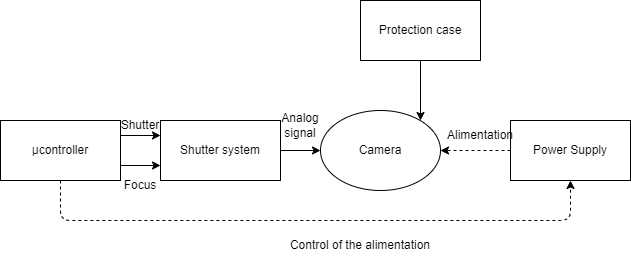
\includegraphics[width=0.9\textwidth]{\currfiledir/figures/camera_diagram.png}
    \caption{Architecture of the system surrounding the camera}
\end{figure}

The camera need a lens to be mounted on it in order to make it work properly. The calculations realized show the lens should be a lens with a focal length between 45 and 150 mm.

Here is the calculation:

\begin{figure}[!h]
    \centering
    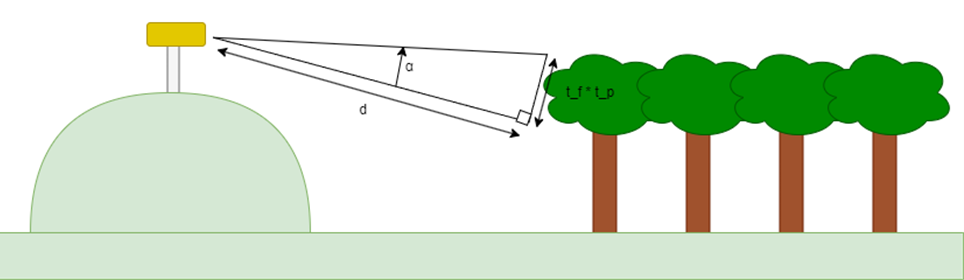
\includegraphics[width=0.85\textwidth]{\currfiledir/figures/calculation_schema.png}
    \caption{Schematic to calculate the focal length for the camera.}
\end{figure}

\noindent\(\alpha\): lens angle of the field of a (to calculate)\\
\(d\): distance between our system and trees (equal to 300 metres)\\
\(t_f\): size of a leaf, estimated to be 5,5 centimetres.\\
\(t_p\): height of the image, which corresponds to 1024 pixels.\\

\noindent According to the trigonometric formulas: \(\alpha=arctan\left(\frac{t_f*t_p}{d}\right)=32,4\textdegree\)

\newpage
%Schematic of different focal lengths
\begin{figure}[!h]
    \centering
    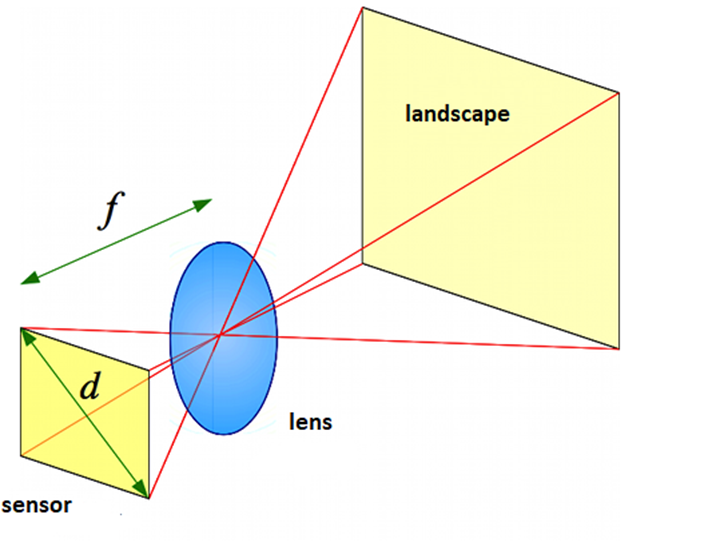
\includegraphics[width=0.75\textwidth]{\currfiledir/figures/calculation.png}
    \caption{Link between angle of view and focal length}
    \cite{focal_length}
\end{figure}

The field of view angle \((\alpha\)) horizontally, corresponding to the length (L) of the sensor, is given by the following formula:
% f=L/(2*tan⁡(α/2) )
\begin{equation}
    f=\frac{L}{2*tan\left(\frac{\alpha}{2}\right)}
\end{equation}

\noindent Where:\\
L: length of the sensor in mm\\
f: focal distance of the lens in mm\\
\(\alpha\): lens angle of the field of view\\
It is obtained: f = 117 mm\\

The equivalent focal length of a Micro 4/3 lens with a field of view of 32.4 degrees is approximately 117 mm.\\


\noindent According to the graph above, we should choose a lens between 100 and 200 mm. The smaller the angle of view (high focal length), the greater the magnification (long focal lengths will give the impression of being closer to the scene captured).\\
Our goal is not to visualize each leaf but each branch so a lens with a focal length of 175 mm will be sufficient for our project.\\
We have therefore selected this objective: \url{https://www.m43lenses.com/panasonic-45-175mm-f4-5.6/}
\newpage
\subsection{Use case}

% \begin{figure}[!h]
%     \centering
%     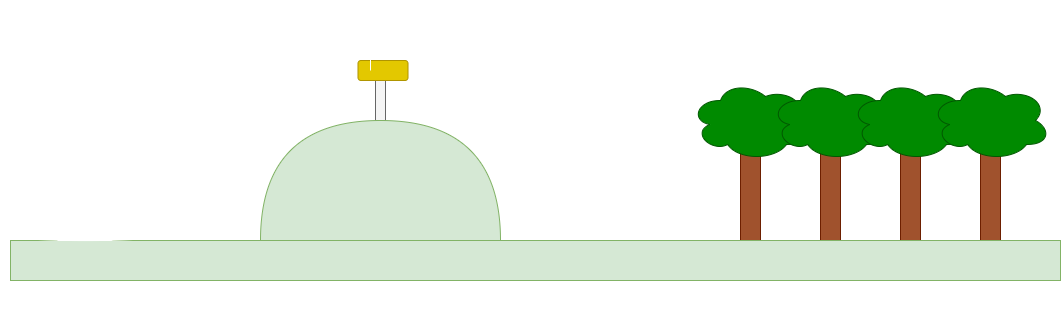
\includegraphics[width=1\textwidth]{\currfiledir/figures/use_case.png}
%     \caption{Use case of the system}
%     \label{fig:forest2}
% \end{figure}


The use case would be as following:
The researchers come once to install the system on a pole on a hill, in front of the group of trees they want to observe. The system would then be placed in the desired location within the forest. The system would be sending data to researchers to ensure that it is functioning properly and that the pictures being taken are of high quality. After 3 months, the researchers would return to the forest to retrieve the system, the stored pictures, and logs about the system state. Then, the researchers would be able to analyse the images.


\newpage
\begin{figure}[!h]
    \centering
    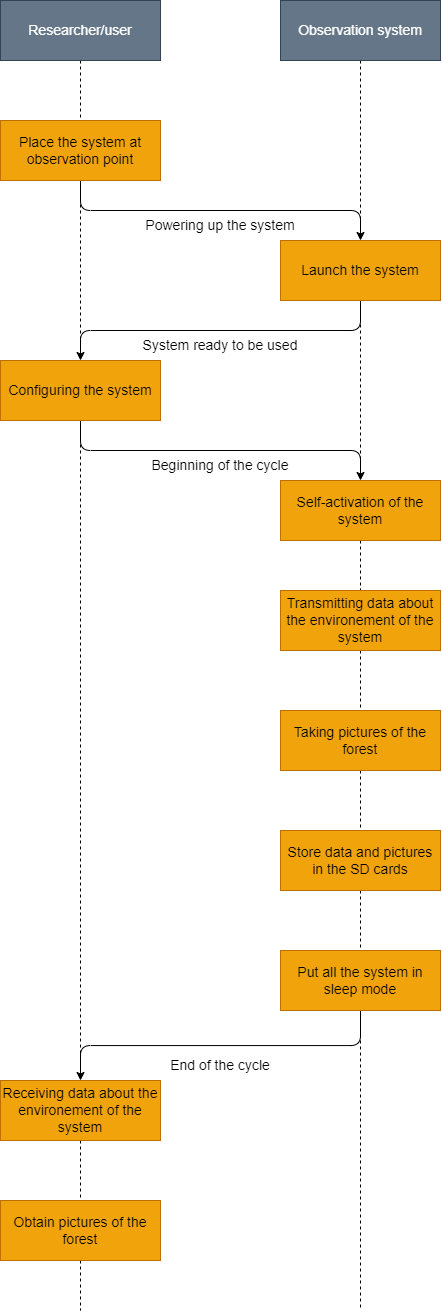
\includegraphics[height=0.95\textheight]{\currfiledir/figures/usage_scenario.png}
    \caption{Picture representing the intended usage scenario for the system.}
\end{figure}

\newpage

\subsection{Functional specifications}

\begin{figure}[!h]
    \centering
    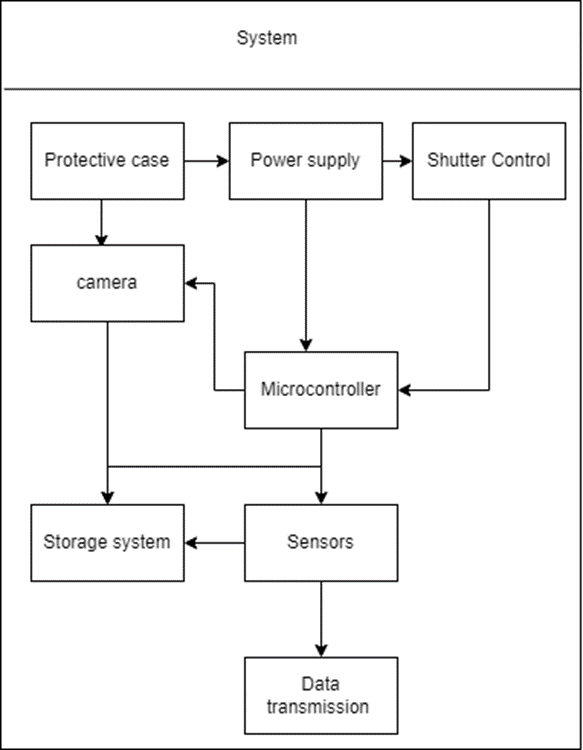
\includegraphics[height=0.5\textheight]{\currfiledir/figures/system.png}
    \caption{Schematic showing different functions interacting inside of the system}
\end{figure}

The diagram illustrates the interconnectivity of these functions, highlighting the relationships and data flow between them. To create a functional system, it is important to ensure that these components are properly integrated and configured to meet the specified technical requirements.

\newpage
\begin{table}[!h]
	\centering
	\begin{tabular}{|c|c|c|c|c|c|}
		\hline
		\rowcolor[HTML]{BFBFBF}
		x                                                  &
		Function                                           &
		Sub-function                                       &
		Criterion                                          &
		Value                                              &
		Flexibility                                          \\ \hline
		F1                                                 &
		\cellcolor[HTML]{CC99FF}Take photos                &
		                                                   &
		                                                   &
		                                                   &
		\cellcolor[HTML]{FFFFFF}{\color[HTML]{FFFFFF} }      \\ \hline
		F1.1                                               &
		                                                   &
		\cellcolor[HTML]{8EA9DB}\begin{tabular}[c]{@{}c@{}}Internal camera \\settings\end{tabular}  &
		                                                   &
		                                                   &
		\\ \hline
		C1.1.1                                             &
		                                                   &
		                                                   &
		\cellcolor[HTML]{A9D08E}Frequency                  &
		\cellcolor[HTML]{FFD966}Once                       &
		\cellcolor[HTML]{ED7D31}2                            \\ \hline
		F1.2                                               &
		                                                   &
		\cellcolor[HTML]{8EA9DB}\begin{tabular}[c]{@{}c@{}}Taking\\ photos regularly\end{tabular}  &
		                                                   &
		                                                   &
		\\ \hline
		C1.2.1                                             &
		                                                   &
		                                                   &
		\cellcolor[HTML]{A9D08E}Frequency                  &
		\cellcolor[HTML]{FFD966}\begin{tabular}[c]{@{}c@{}}2 times a\\ day\end{tabular}  &
		\cellcolor[HTML]{ED7D31}0                            \\ \hline
		F1.3                                               &
		                                                   &
		\cellcolor[HTML]{8EA9DB}\begin{tabular}[c]{@{}c@{}}Taking high-\\ quality photos\end{tabular}  &
		                                                   &
		                                                   &
		\\ \hline
		C1.3.1                                             &
		                                                   &
		                                                   &
		\cellcolor[HTML]{A9D08E}Resolution                 &
		\cellcolor[HTML]{FFD966}1920x1080                    &
		\cellcolor[HTML]{ED7D31}0                            \\ \hline
		C1.3.2                                             &
		                                                   &
		\multicolumn{1}{l|}{}                              &
		\cellcolor[HTML]{A9D08E}Distance                   &
		\cellcolor[HTML]{FFD966}\begin{tabular}[c]{@{}c@{}}300 meters\end{tabular}  &
		\cellcolor[HTML]{ED7D31}0                            \\ \hline
		C1.3.3                                             &
		                                                   &
		\multicolumn{1}{l|}{}                              &
		\cellcolor[HTML]{A9D08E}Fields of view             &
		\cellcolor[HTML]{FFD966}\begin{tabular}[c]{@{}c@{}}32.4°\end{tabular}  &
		\cellcolor[HTML]{ED7D31}1                            \\ \hline 
		F2                                                 &
		\cellcolor[HTML]{CC99FF}\begin{tabular}[c]{@{}c@{}}Possessing an extended\\ battery life\end{tabular}  &
		                                                   &
		                                                   &
		                                                   &
		\\ \hline
		F2.1                                               &
		                                                   &
		\cellcolor[HTML]{8EA9DB}\begin{tabular}[c]{@{}c@{}}Possessing an extended \\battery life\end{tabular}  &
		                                                   &
		                                                   &
		\\ \hline
		C2.1.1                                             &
		                                                   &
		                                                   &
		\cellcolor[HTML]{A9D08E}\begin{tabular}[c]{@{}c@{}}Desired uptime\end{tabular}  &
		\cellcolor[HTML]{FFD966}\(\approx\) 1 year                   &
		\cellcolor[HTML]{ED7D31}1                            \\ \hline
		F3                                                 &
		\cellcolor[HTML]{CC99FF}Storing data               &
		                                                   &
		                                                   &
		                                                   &
		\\ \hline
		F3.1                                               &
		                                                   &
		\cellcolor[HTML]{8EA9DB}Store photos               &
		                                                   &
		                                                   &
		\\ \hline
		C3.1.1                                             &
		                                                   &
		                                                   &
		\cellcolor[HTML]{A9D08E}\begin{tabular}[c]{@{}c@{}}Picture-dedicated \\storage space\end{tabular}  &
		\cellcolor[HTML]{FFD966}\textgreater 16 Go         &
		\cellcolor[HTML]{ED7D31}1                            \\ \hline
		F3.2                                               &
		                                                   &
		\cellcolor[HTML]{8EA9DB}\begin{tabular}[c]{@{}c@{}}Storing  \\ information on \\ the device state\end{tabular} &
		                                                   &
		                                                   &
		\\ \hline
		C3.2.1                                             &
		                                                   &
		                                                   &
		\cellcolor[HTML]{A9D08E}\begin{tabular}[c]{@{}c@{}}Information-dedicated \\ storage  \\ space\end{tabular} &
		\cellcolor[HTML]{FFD966}16 Mo                      &
		\cellcolor[HTML]{ED7D31}3                            \\ \hline
		C3.2.2                                             &
		                                                   &
		                                                   &
		\cellcolor[HTML]{A9D08E}\begin{tabular}[c]{@{}c@{}}Logging period\end{tabular} &
		\cellcolor[HTML]{FFD966}\(\approx\) 1 months                 &
		\cellcolor[HTML]{ED7D31}3                            \\ \hline
		F4                                                 &
		\cellcolor[HTML]{CC99FF}\begin{tabular}[c]{@{}c@{}}Conveying system \\status information\end{tabular} &
		                                                   &
		                                                   &
		                                                   &
		\\ \hline
		F4.1                                               &
		                                                   &
		\cellcolor[HTML]{8EA9DB}Collecting information             &
		                                                   &
		                                                   &
		\\ \hline
		C4.1.1                                             &
		                                                   &
		                                                   &
		\cellcolor[HTML]{A9D08E}\begin{tabular}[c]{@{}c@{}}Remaining battery\\charge percentage\end{tabular} &
		\cellcolor[HTML]{FFD966}\begin{tabular}[c]{@{}c@{}}Error margin \\ of 10\%\end{tabular} &
		\cellcolor[HTML]{ED7D31}2                            \\ \hline
	\end{tabular}
\end{table}

\newpage

% Please add the following required packages to your document preamble:
% \usepackage{multirow}
% \usepackage[table,xcdraw]{xcolor}
% If you use beamer only pass "xcolor=table" option, i.e. \documentclass[xcolor=table]{beamer}
% Please add the following required packages to your document preamble:
% \usepackage{multirow}
% \usepackage[table,xcdraw]{xcolor}
% If you use beamer only pass "xcolor=table" option, i.e. \documentclass[xcolor=table]{beamer}
\begin{table}[!h]
    \centering
    \begin{tabular}{|c|c|c|c|c|c|}
    \hline
     &
       &
       &
      \cellcolor[HTML]{A9D08E} &
      \cellcolor[HTML]{FFD966}\begin{tabular}[c]{@{}c@{}}0°C to 5\\ 0°C\end{tabular} &
      \cellcolor[HTML]{ED7D31}2 \\ \cline{5-6} 
    \multirow{-2}{*}{C4.1.2} &
      \multirow{-2}{*}{} &
      \multirow{-2}{*}{} &
      \multirow{-2}{*}{\cellcolor[HTML]{A9D08E}Temperature} &
      \cellcolor[HTML]{FFD966}\begin{tabular}[c]{@{}c@{}}Precision \\ of 1°C\end{tabular} &
      \cellcolor[HTML]{ED7D31}0 \\ \hline
    C4.1.3 &
       &
       &
      \cellcolor[HTML]{A9D08E}Humidity &
      \cellcolor[HTML]{FFD966}\begin{tabular}[c]{@{}c@{}}80 to \\ 100\%\end{tabular} &
      \cellcolor[HTML]{ED7D31}2 \\ \hline
    C4.1.4 &
       &
       &
      \cellcolor[HTML]{A9D08E}\begin{tabular}[c]{@{}c@{}}Remaining\\  storage\\  space\end{tabular} &
      \cellcolor[HTML]{FFD966}\begin{tabular}[c]{@{}c@{}}Warning \\ at 90\%\end{tabular} &
      \cellcolor[HTML]{ED7D31}2 \\ \hline
    C4.1.5 &
       &
       &
      \cellcolor[HTML]{A9D08E}\begin{tabular}[c]{@{}c@{}}Device \\ motion\end{tabular} &
      \cellcolor[HTML]{FFD966}\begin{tabular}[c]{@{}c@{}}Precision : \\ ± 1cm | \\ ± 1°\end{tabular} &
      \cellcolor[HTML]{ED7D31}1 \\ \hline
    F4.2 &
       &
      \cellcolor[HTML]{8EA9DB}\begin{tabular}[c]{@{}c@{}}Transmitting \\ data remotely\end{tabular} &
       &
       &
       \\ \hline
    C4.2.1 &
       &
       &
      \cellcolor[HTML]{A9D08E}Range &
      \cellcolor[HTML]{FFD966}\(\geq\) 10km &
      \cellcolor[HTML]{ED7D31}1 \\ \hline
    F5 &
      \cellcolor[HTML]{CC99FF}\begin{tabular}[c]{@{}c@{}}Working in a\\  specific \\ environment\end{tabular} &
       &
       &
       &
       \\ \hline
    F5.1 &
       &
      \cellcolor[HTML]{8EA9DB}\begin{tabular}[c]{@{}c@{}}Resisting Central \\ African climate\end{tabular} &
       &
       &
       \\ \hline
    C5.1.1 &
       &
       &
      \cellcolor[HTML]{A9D08E}\begin{tabular}[c]{@{}c@{}}Humidity \\ and fog\end{tabular} &
      \cellcolor[HTML]{FFD966}\begin{tabular}[c]{@{}c@{}}\textgreater 90\% of \\ humidity\end{tabular} &
      \cellcolor[HTML]{ED7D31}0 \\ \hline
    C5.1.2 &
       &
       &
      \cellcolor[HTML]{A9D08E}Temperature &
      \cellcolor[HTML]{FFD966}20°C to 35°C &
      \cellcolor[HTML]{ED7D31}0 \\ \hline
    C5.1.3 &
       &
       &
      \cellcolor[HTML]{A9D08E}Rain &
      \cellcolor[HTML]{FFD966}\begin{tabular}[c]{@{}c@{}}equivalent to\\ IPX4\end{tabular} &
      \cellcolor[HTML]{ED7D31}0 \\ \hline
    \cellcolor[HTML]{FFFFFF}F5.2 &
      \cellcolor[HTML]{FFFFFF} &
      \cellcolor[HTML]{8EA9DB}Size &
       &
       &
       \\ \hline
    \cellcolor[HTML]{FFFFFF}C5.2.1 &
      \cellcolor[HTML]{FFFFFF} &
       &
      \cellcolor[HTML]{A9D08E}Dimensions &
      \cellcolor[HTML]{FFD966}200x300x150 mm &
      \cellcolor[HTML]{ED7D31}2 \\ \hline
    \cellcolor[HTML]{FFFFFF}F5.3 &
      \cellcolor[HTML]{FFFFFF} &
      \cellcolor[HTML]{8EA9DB}Weight &
       &
       &
       \\ \hline
    \cellcolor[HTML]{FFFFFF}C5.3.1 &
      \cellcolor[HTML]{FFFFFF} &
       &
      \cellcolor[HTML]{A9D08E}Mass &
      \cellcolor[HTML]{FFD966}4 kg &
      \cellcolor[HTML]{ED7D31}1 \\ \hline
    \cellcolor[HTML]{FFFFFF}F5.4 &
      \cellcolor[HTML]{FFFFFF} &
      \cellcolor[HTML]{8EA9DB}\begin{tabular}[c]{@{}c@{}}Installation\end{tabular} &
       &
       &
       \\ \hline
    \cellcolor[HTML]{FFFFFF}C5.4.1 &
      \cellcolor[HTML]{FFFFFF} &
       &
      \cellcolor[HTML]{A9D08E}\begin{tabular}[c]{@{}c@{}}Relevant stand \\ or platform\end{tabular} &
      \cellcolor[HTML]{FFD966}??? &
      \cellcolor[HTML]{ED7D31}1 \\ \hline
    \end{tabular}
\end{table}
\tab\tab




%table des figures
\newpage
%configuration de l'affichage pour les sous figure (profondeur)
\setcounter{lofdepth}{2}
%table des figures
\listoffigures


%bibliographie
\newpage{}
%le \phantomsection{} permet de regler un bug sur les sommaire qui ne ramène pas a la bonne page
\phantomsection{}
\addcontentsline{toc}{section}{Reference}
\DeclareFieldFormat{labelnumberwidth}{}
\setlength{\biblabelsep}{0pt}
\nocite{*}
\printbibliography{}

%annexe
\newpage
%le \phantomsection{} permet de regler un bug sur les sommaire qui ne ramène pas a la bonne page
\phantomsection{}
%section sans numéro
\section*{Appendices}
%ajouter quand même la section dans le sommaire
\addcontentsline{toc}{section}{Appendices}

\subsection*{Github repository}
Everything we used (code,documentation,schematic ...) is available on our GitHub repository on this link : \url{https://github.com/RedCoal27/4AGPSE-Forest-Watch}

\subsection*{Horned beast diagram of the system}
\begin{figure}[!h]
    \centering
    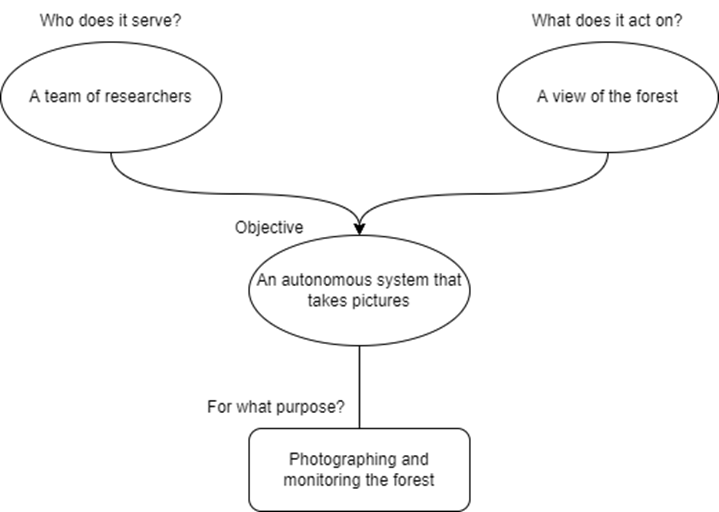
\includegraphics[width=0.6\textwidth]{\currfiledir/figures/horned.png}
    \caption{Horned beast diagram of the system}
\end{figure}

\subsection*{Horned beast diagram for Lora}
\begin{figure}[!h]
    \centering
    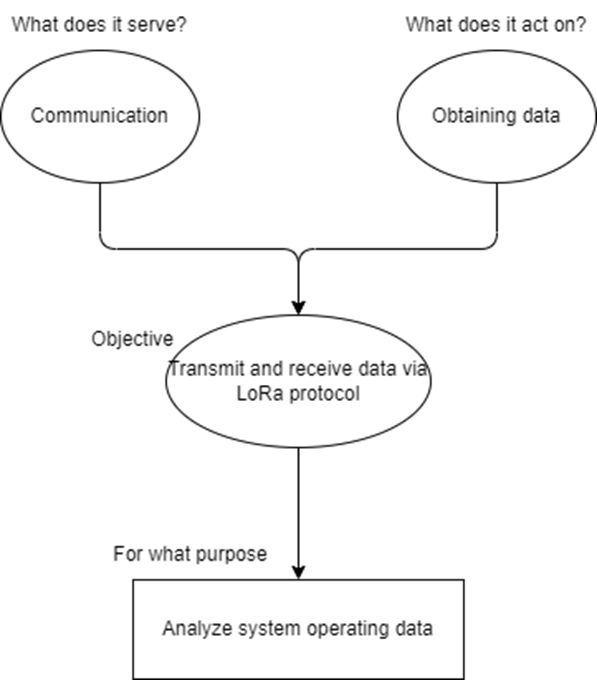
\includegraphics[width=0.48\textwidth]{\currfiledir/figures/horned_lora.png}
    \caption{Horned beast diagram for Lora}
\end{figure}

\newpage
\subsection*{Self-assessment:}
\newpage
\subsubsection*{Krasulja Florian}
I was part of the team that worked on the design and implementation of an autonomous system for taking pictures of a tropical forest in Gabon for research purposes. As a member of the team, I was responsible for the following tasks:

\begin{itemize}
    \item Product design: I have gained experience in designing a product that meets the specific requirements and constraints of the project, such as durability, waterproofing, ventilation, and ease of access.
    \item Technical drawing and 3D modeling: I have improved my skills in using technical drawing software and 3D modeling software to create detailed and accurate designs of the case.
    \item Project management: I have gained experience in working in a team and coordinating with other members to ensure that the design of the case is completed on schedule.
    \item Communication: I have improved my ability to communicate my ideas and designs effectively to the rest of the team, and to explain the reasoning behind my design choices.
\end{itemize}

Overall, I believe that my contribution to the design of the case has been significant, and I am proud of the final product. I believe that my experience in this project will be valuable in future projects, both in terms of technical skills and experience in project management.\\

\begin{table}[!h]
    \centering
    \begin{tabular}{|cc|}
    \hline
    \multicolumn{2}{|c|}{\cellcolor[HTML]{9698ED}Florian}                 \\ \hline
    \multicolumn{1}{|c|}{3D Drawing/Printing} & Beginner → Intermediate + \\ \hline
    \multicolumn{1}{|c|}{Enclosure}           & 0→ Intermediate           \\ \hline
    \multicolumn{1}{|c|}{Imaging system}      & Beginner→ Intermediate    \\ \hline
    \multicolumn{1}{|c|}{Teamwork}            & Beginner → Intermediate   \\ \hline
    \end{tabular}
\end{table}
\newpage
\subsubsection*{Maillet Alexandre}
As a member of the team responsible for the design and implementation of an autonomous system for taking pictures of a tropical forest in Gabon for research purposes, I was responsible for the alimentation part of the system. My role in the project included the following tasks:

\begin{itemize}
\item Alimentation system design: I have gained experience in designing an alimentation system that meets the specific requirements and constraints of the project, such as the use of a 12V 2,3Ah lead battery, a 10w solar panel, a sun voltage regulator, and a LM317 to regulate the voltage to approximately 8V.
\item Voltage regulation: I have improved my skills in using LM317 and other regulators to ensure that the voltage supplied to the camera and microcontroller is within the proper range.
\item Project management: I have gained experience in working in a team and coordinating with other members to ensure that the alimentation system is completed on schedule.
\item Communication: I have improved my ability to communicate my ideas and designs effectively to the rest of the team, and to explain the reasoning behind my design choices.
\end{itemize}

Although my contribution to the project was significant, I believe that we could have worked harder on the project. I think that if we put more effort into it, we could have improved the final product even more. Nevertheless, I believe that my experience in this project will be valuable in future projects, both in terms of technical skills and experience in project management.\\


% Please add the following required packages to your document preamble:
% \usepackage[table,xcdraw]{xcolor}
% If you use beamer only pass "xcolor=table" option, i.e. \documentclass[xcolor=table]{beamer}
\begin{table}[!h]
    \centering
    \begin{tabular}{|cc|}
    \hline
    \multicolumn{2}{|c|}{\cellcolor[HTML]{FF0000}Alexandre}                 \\ \hline
    \multicolumn{1}{|c|}{Arduino/C++}       & Intermediate → Advanced       \\ \hline
    \multicolumn{1}{|c|}{PCB Manufacturing} & Intermediate+ → Intermediate+ \\ \hline
    \multicolumn{1}{|c|}{Electronics}       & Intermediate+→ Advanced       \\ \hline
    \multicolumn{1}{|c|}{Team Management}   & 0 → Beginner                  \\ \hline
    \multicolumn{1}{|c|}{Teamwork}          & Beginner → Intermediate       \\ \hline
    \end{tabular}
\end{table}
\newpage
\subsubsection*{DE SOUSA CARDOSO Raimundo Vitor}
The first part of this project allowed me to learn and develop competencies in the areas in which I worked towards the development of the system. Especially those related to modelling and project planning, as well as the communication part via LoRa protocol.
In the part involving planning, I could learn how to organize and detail a project before its execution. I was able to do different analyses, functional, risk, and process, some of them using the Cappella software. 
In the communication via LoRa protocol part, I could understand how the architecture of this technology works. I applied the knowledge obtained in classes to perform a communication via UART between the microcontroller and the LoRa/GPS HAT, also providing a learning and code development for programming this function.
Finally, by working alongside a fantastic team, I was able to develop my teamwork skills, especially in an environment where I was communicating using a foreign language. I learned a lot by debating ideals, discussing problems, pointing out solutions, and presenting our project to teachers and students.



\begin{table}[!h]
    \centering
    \begin{tabular}{|cc|}
    \hline
    \multicolumn{2}{|c|}{\cellcolor[HTML]{32CB00}Raimundo}           \\ \hline
    \multicolumn{1}{|c|}{LoRa}        & 0 →  Intermediate            \\ \hline
    \multicolumn{1}{|c|}{Arduino/C++} & Beginner → Intermediate      \\ \hline
    \multicolumn{1}{|c|}{Raspbian}    & 0 → Intermediate             \\ \hline
    \multicolumn{1}{|c|}{Teamwork}    & Intermediate → Intermediate+ \\ \hline
    \end{tabular}
\end{table}
\newpage
\subsubsection*{Abdelkrim Darrys}
% While working on this project, I contributed on many aspects:
% •	Research: In this project, I took part on research about components and methods. For example, I researched components to buy for the project alongside other team members. I also made research on how remote shutter systems work to reproduce it.

% •	Project management: This project permitted me to improve my skills in project management and communication with my colleagues. 

% •	Documentation: While writing documentation for the project, it helped me to better understand what my colleagues were doing and to write technical documents. I also documented what we were doing each time we were working on the project.

While working on this project, I contributed on many aspects:
\begin{itemize}
    \item Research: In this project, I took part on research about components and methods. For example, I researched components to buy for the project alongside other team members. I also made research on how remote shutter systems work to reproduce it.
    \item Project management: This project permitted me to improve my skills in project management and communication with my colleagues. 
    \item Documentation: While writing documentation for the project, it helped me to better understand what my colleagues were doing and to write technical documents. I also documented what we were doing each time we were working on the project.
\end{itemize}


\begin{table}[!h]
    \centering
    \begin{tabular}{|cc|}
    \hline
    \multicolumn{2}{|c|}{\cellcolor[HTML]{3531FF}Darrys}                \\ \hline
    \multicolumn{1}{|c|}{Arduino/C++}    & Beginner → Intermediate      \\ \hline
    \multicolumn{1}{|c|}{Electronics}    & Intermediate → Intermediate+ \\ \hline
    \multicolumn{1}{|c|}{Imaging System} & 0 → Intermediate             \\ \hline
    \multicolumn{1}{|c|}{Teamwork}       & Intermediate → Intermediate+ \\ \hline
    \end{tabular}
\end{table}






%\newpage

%annexes
%\newpage
%le \phantomsection{} permet de regler un bug sur les sommaire qui ne ramène pas a la bonne page
\phantomsection{}
%section sans numéro
\section*{Appendices}
%ajouter quand même la section dans le sommaire
\addcontentsline{toc}{section}{Appendices}

\subsection*{Github repository}
Everything we used (code,documentation,schematic ...) is available on our GitHub repository on this link : \url{https://github.com/RedCoal27/4AGPSE-Forest-Watch}

\subsection*{Horned beast diagram of the system}
\begin{figure}[!h]
    \centering
    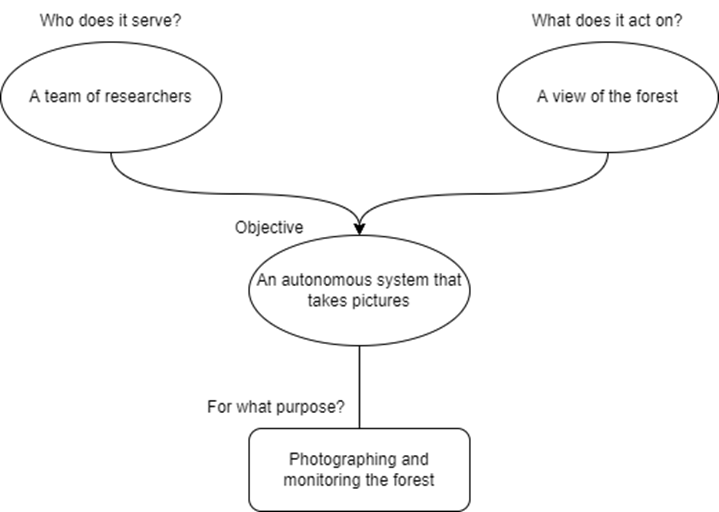
\includegraphics[width=0.6\textwidth]{\currfiledir/figures/horned.png}
    \caption{Horned beast diagram of the system}
\end{figure}

\subsection*{Horned beast diagram for Lora}
\begin{figure}[!h]
    \centering
    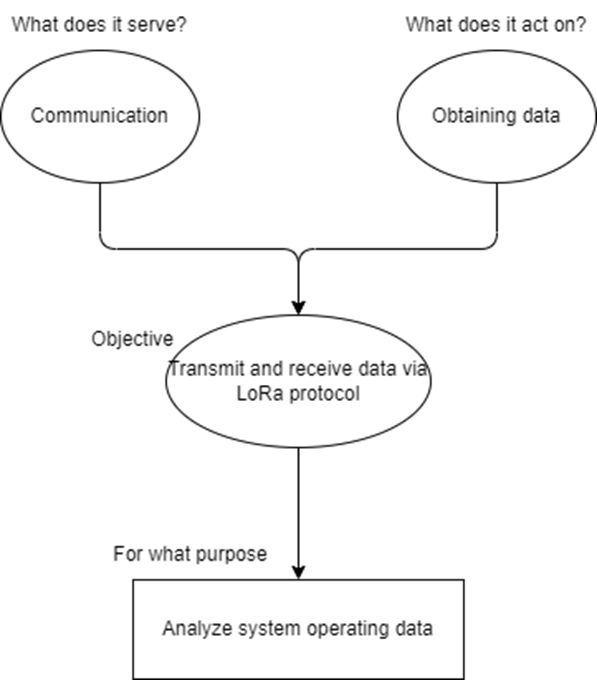
\includegraphics[width=0.48\textwidth]{\currfiledir/figures/horned_lora.png}
    \caption{Horned beast diagram for Lora}
\end{figure}

\newpage
\subsection*{Self-assessment:}
\newpage
\subsubsection*{Krasulja Florian}
I was part of the team that worked on the design and implementation of an autonomous system for taking pictures of a tropical forest in Gabon for research purposes. As a member of the team, I was responsible for the following tasks:

\begin{itemize}
    \item Product design: I have gained experience in designing a product that meets the specific requirements and constraints of the project, such as durability, waterproofing, ventilation, and ease of access.
    \item Technical drawing and 3D modeling: I have improved my skills in using technical drawing software and 3D modeling software to create detailed and accurate designs of the case.
    \item Project management: I have gained experience in working in a team and coordinating with other members to ensure that the design of the case is completed on schedule.
    \item Communication: I have improved my ability to communicate my ideas and designs effectively to the rest of the team, and to explain the reasoning behind my design choices.
\end{itemize}

Overall, I believe that my contribution to the design of the case has been significant, and I am proud of the final product. I believe that my experience in this project will be valuable in future projects, both in terms of technical skills and experience in project management.\\

\begin{table}[!h]
    \centering
    \begin{tabular}{|cc|}
    \hline
    \multicolumn{2}{|c|}{\cellcolor[HTML]{9698ED}Florian}                 \\ \hline
    \multicolumn{1}{|c|}{3D Drawing/Printing} & Beginner → Intermediate + \\ \hline
    \multicolumn{1}{|c|}{Enclosure}           & 0→ Intermediate           \\ \hline
    \multicolumn{1}{|c|}{Imaging system}      & Beginner→ Intermediate    \\ \hline
    \multicolumn{1}{|c|}{Teamwork}            & Beginner → Intermediate   \\ \hline
    \end{tabular}
\end{table}
\newpage
\subsubsection*{Maillet Alexandre}
As a member of the team responsible for the design and implementation of an autonomous system for taking pictures of a tropical forest in Gabon for research purposes, I was responsible for the alimentation part of the system. My role in the project included the following tasks:

\begin{itemize}
\item Alimentation system design: I have gained experience in designing an alimentation system that meets the specific requirements and constraints of the project, such as the use of a 12V 2,3Ah lead battery, a 10w solar panel, a sun voltage regulator, and a LM317 to regulate the voltage to approximately 8V.
\item Voltage regulation: I have improved my skills in using LM317 and other regulators to ensure that the voltage supplied to the camera and microcontroller is within the proper range.
\item Project management: I have gained experience in working in a team and coordinating with other members to ensure that the alimentation system is completed on schedule.
\item Communication: I have improved my ability to communicate my ideas and designs effectively to the rest of the team, and to explain the reasoning behind my design choices.
\end{itemize}

Although my contribution to the project was significant, I believe that we could have worked harder on the project. I think that if we put more effort into it, we could have improved the final product even more. Nevertheless, I believe that my experience in this project will be valuable in future projects, both in terms of technical skills and experience in project management.\\


% Please add the following required packages to your document preamble:
% \usepackage[table,xcdraw]{xcolor}
% If you use beamer only pass "xcolor=table" option, i.e. \documentclass[xcolor=table]{beamer}
\begin{table}[!h]
    \centering
    \begin{tabular}{|cc|}
    \hline
    \multicolumn{2}{|c|}{\cellcolor[HTML]{FF0000}Alexandre}                 \\ \hline
    \multicolumn{1}{|c|}{Arduino/C++}       & Intermediate → Advanced       \\ \hline
    \multicolumn{1}{|c|}{PCB Manufacturing} & Intermediate+ → Intermediate+ \\ \hline
    \multicolumn{1}{|c|}{Electronics}       & Intermediate+→ Advanced       \\ \hline
    \multicolumn{1}{|c|}{Team Management}   & 0 → Beginner                  \\ \hline
    \multicolumn{1}{|c|}{Teamwork}          & Beginner → Intermediate       \\ \hline
    \end{tabular}
\end{table}
\newpage
\subsubsection*{DE SOUSA CARDOSO Raimundo Vitor}
The first part of this project allowed me to learn and develop competencies in the areas in which I worked towards the development of the system. Especially those related to modelling and project planning, as well as the communication part via LoRa protocol.
In the part involving planning, I could learn how to organize and detail a project before its execution. I was able to do different analyses, functional, risk, and process, some of them using the Cappella software. 
In the communication via LoRa protocol part, I could understand how the architecture of this technology works. I applied the knowledge obtained in classes to perform a communication via UART between the microcontroller and the LoRa/GPS HAT, also providing a learning and code development for programming this function.
Finally, by working alongside a fantastic team, I was able to develop my teamwork skills, especially in an environment where I was communicating using a foreign language. I learned a lot by debating ideals, discussing problems, pointing out solutions, and presenting our project to teachers and students.



\begin{table}[!h]
    \centering
    \begin{tabular}{|cc|}
    \hline
    \multicolumn{2}{|c|}{\cellcolor[HTML]{32CB00}Raimundo}           \\ \hline
    \multicolumn{1}{|c|}{LoRa}        & 0 →  Intermediate            \\ \hline
    \multicolumn{1}{|c|}{Arduino/C++} & Beginner → Intermediate      \\ \hline
    \multicolumn{1}{|c|}{Raspbian}    & 0 → Intermediate             \\ \hline
    \multicolumn{1}{|c|}{Teamwork}    & Intermediate → Intermediate+ \\ \hline
    \end{tabular}
\end{table}
\newpage
\subsubsection*{Abdelkrim Darrys}
% While working on this project, I contributed on many aspects:
% •	Research: In this project, I took part on research about components and methods. For example, I researched components to buy for the project alongside other team members. I also made research on how remote shutter systems work to reproduce it.

% •	Project management: This project permitted me to improve my skills in project management and communication with my colleagues. 

% •	Documentation: While writing documentation for the project, it helped me to better understand what my colleagues were doing and to write technical documents. I also documented what we were doing each time we were working on the project.

While working on this project, I contributed on many aspects:
\begin{itemize}
    \item Research: In this project, I took part on research about components and methods. For example, I researched components to buy for the project alongside other team members. I also made research on how remote shutter systems work to reproduce it.
    \item Project management: This project permitted me to improve my skills in project management and communication with my colleagues. 
    \item Documentation: While writing documentation for the project, it helped me to better understand what my colleagues were doing and to write technical documents. I also documented what we were doing each time we were working on the project.
\end{itemize}


\begin{table}[!h]
    \centering
    \begin{tabular}{|cc|}
    \hline
    \multicolumn{2}{|c|}{\cellcolor[HTML]{3531FF}Darrys}                \\ \hline
    \multicolumn{1}{|c|}{Arduino/C++}    & Beginner → Intermediate      \\ \hline
    \multicolumn{1}{|c|}{Electronics}    & Intermediate → Intermediate+ \\ \hline
    \multicolumn{1}{|c|}{Imaging System} & 0 → Intermediate             \\ \hline
    \multicolumn{1}{|c|}{Teamwork}       & Intermediate → Intermediate+ \\ \hline
    \end{tabular}
\end{table}




\end{document}


%====================== FIN DU DOCUMENT ======================